% Complete cumulative LaTeX source for the named public edition.
% Build from releases/ inside the extracted source bundle; dependencies are under ../upstream/.
% XeLaTeX and the bundled guard workflow are documented in README.md.
\documentclass[12pt,a4paper,oneside]{report}
\usepackage[margin=24mm]{geometry}
\usepackage{fontspec}
\setmainfont[Script=Arabic]{Amiri}
\newfontfamily\latinfont{Latin Modern Roman}
\usepackage{amsmath,amssymb,amsthm,mathrsfs,nicefrac}
\usepackage{xparse,graphicx,tikz,xcolor}
\usepackage[authoryear]{natbib}
\usepackage[unicode,colorlinks,linkcolor=blue]{hyperref}
\usepackage{bidi}
\hypersetup{pdftitle={OpenLogic Pashto Pakistan - Sets and Relations},pdfauthor={Open Logic Project; machine translation adaptation},pdfsubject={Partial edition: two complete chapters; full 722-unit edition in progress}}
\definecolor{oldiagcolorA}{RGB}{38,89,117}
\definecolor{oldiagcolorB}{RGB}{189,83,41}
\definecolor{oldiagcolorC}{RGB}{44,115,104}
\newcommand{\Setabs}[2]{\{#1 : #2\}}
\newcommand{\Pow}[1]{\wp(#1)}
\newcommand{\Nat}{\mathbb{N}}
\newcommand{\Int}{\mathbb{Z}}
\newcommand{\Rat}{\mathbb{Q}}
\newcommand{\Real}{\mathbb{R}}
\newcommand{\PosInt}{\mathbb{Z}^{+}}
\newcommand{\Bin}{\mathbb{B}}
\newcommand{\tuple}[1]{\langle #1\rangle}
\newcommand{\len}[1]{\mathrm{len}(#1)}
\newcommand{\lif}{\mathbin{\rightarrow}}
\newcommand{\liff}{\mathbin{\leftrightarrow}}
\newcommand{\Id}[1]{\mathord{\mathrm{Id}_{#1}}}
\newcommand{\emptyseq}{\Lambda}
\newcommand{\equivrep}[2]{[#1]_{#2}}
\newcommand{\equivclass}[2]{#1/_{\!{#2}}}
\newcommand{\funrestrictionto}[2]{#1\mathord{\restriction}_{#2}}
\newcommand{\funimage}[2]{#1[#2]}
\newcommand{\olfileid}[3]{\gdef\pspart{#1}\gdef\pschapter{#2}\gdef\pssection{#3}}
\newcommand{\olchapter}[3]{\gdef\pspart{#1}\gdef\pschapter{#2}\gdef\pssection{}\chapter{#3}\label{#1:#2::chap}}
\newcommand{\olsection}[1]{\section{#1}\label{\pspart:\pschapter:\pssection:sec}}
\newcommand{\ollabel}[1]{\label{\pspart:\pschapter:\pssection:#1}}
% Match upstream's right-relative optional arguments, including explicit empty values.
\NewDocumentCommand{\olref}{o o o m}{\begingroup
\IfNoValueTF{#1}{\def\pskey{\pspart:\pschapter:\pssection:#4}}{
  \IfNoValueTF{#2}{\def\pskey{\pspart:\pschapter:#1:#4}}{
    \IfNoValueTF{#3}{\def\pskey{\pspart:#1:#2:#4}}{\def\pskey{#1:#2:#3:#4}}}}
\LR{\ref{\pskey}}\endgroup}
\NewDocumentCommand{\oliflabeldef}{m m m}{\ifcsname r@#1\endcsname #2\else #3\fi}
\newcommand{\olasset}[1]{\centering\begin{LTR}\centering\resizebox{.46\textwidth}{!}{\input{../upstream/#1}}\end{LTR}}
\newenvironment{explain}{}{}
\newenvironment{intro}{}{}
\newenvironment{digress}{\par\medskip}{\par\medskip}
\newenvironment{tagblock}[1]{}{}
\newtheorem{defn}{تعريف}[section]
\newtheorem{ex}[defn]{بېلګه}
\newtheorem{prop}[defn]{قضيه}
\newtheorem{thm}[defn]{قضيه}
\newtheorem{prob}[defn]{تمرين}
\renewcommand{\proofname}{ثبوت}
\renewcommand{\figurename}{شکل}
\renewcommand{\chaptername}{باب}
\renewcommand{\contentsname}{فهرست}
\renewcommand{\bibname}{\RL{\normalfont سرچينې}}
\setlength{\parindent}{0pt}
\setlength{\parskip}{6pt}
\emergencystretch=2em
\linespread{1.18}
\begin{document}
\setRTL
\begin{titlepage}
\begin{center}
\vspace*{25mm}
{\Huge خلاص منطق}\par\bigskip
{\Large پښتو — پاکستان}\par\bigskip
{\LARGE سټونه او اړيکې}\par\bigskip
د ماشيني ژباړې د روان کار نسخه
\end{center}
\bigskip
په دې لوستيزه نسخه کښې دوه بشپړ بابونه شامل دي۔ د ټول کتاب ژباړه لا
روانه ده۔ د سرچينو شواهد، اصطلاحي پرېکړې او د کتنې حدود له دې نسخې
سره په ملګري موادو کښې ثبت دي۔
\begin{LTR}\latinfont\small
An independent machine translation of the Open Logic Project, revision\\
\texttt{9620cc73f9c8e0ad003c514a5d3748f29611c4c0}.\par
This reader contains the complete sets and relations chapters (16 source
units). The source bundle also includes three front matter and import-driver
drafts: 19 of 722 source units in total. The full edition remains in progress.
Native Pakistani prose is primary; Afghan Pashto references are labelled
regional comparators. Terminology remains provisional where exact technical
attestation is sparse. This is not a claim of native-reader review.

Original text and adaptation: Creative Commons Attribution 4.0 International,
subject to the component notices preserved with upstream source.
No upstream endorsement is implied.
\href{https://openlogicproject.org/}{Open Logic Project}.\quad
\href{https://github.com/KokunoYumeto/OpenLogic-translations}{Translation catalogue}.\quad
\href{https://doi.org/10.5281/zenodo.22307197}{Edition version lineage}.
\end{LTR}
\end{titlepage}
\tableofcontents
\clearpage

\olchapter{sfr}{set}{سټونه}


\olfileid{sfr}{set}{bas}
\olsection{د غړو له مخې برابري}

\emph{سټ} د څيزونو يوه ټولګه ده چې د يوه څيز په توګه ورته کتل کېږي۔ هغه څيزونه چې سټ ترې جوړ وي، د سټ \emph{عناصر} يا \emph{غړي} بللے شي۔ که \LR{$x$} د يو سټ~\LR{$A$} غړے وي، \LR{$x \in A$} ليکو؛ که نۀ وي، \LR{$x \notin A$} ليکو۔ هغه سټ چې هېڅ غړي نۀ لري، \emph{تش} سټ بللے شي او په ``\LR{$\emptyset$}'' ښودلے کېږي۔

\begin{explain}
دا مهمه نۀ ده چې سټ څنګه \emph{ټاکو}، د هغۀ غړي څنګه \emph{ترتيبوو}، يا په رښتيا د هغۀ غړي \emph{څو ځله} شمارو۔ يوازې دا مهم دي چې د هغۀ غړي کوم دي۔ دا خبره په لاندې اصل کښې راټولوو۔
\end{explain}

\begin{defn}[د غړو له مخې برابري]
  که \LR{$A$} او \LR{$B$} سټونه وي، نو \LR{$A = B$} هله او يوازې هله وي چې د~\LR{$A$} هر غړے د~\LR{$B$} هم غړے وي، او برعکس۔
\end{defn}

د غړو له مخې برابري د ځينو نښو د کارولو جواز راکوي۔ په عمومي توګه، چې کله ځينې څيزونه \LR{$a_{1}$}، \dots، \LR{$a_{n}$} ولرو، نو \LR{$\{a_{1}, \dots, a_{n}\}$} \emph{هم هغه} سټ دے چې غړي ئې \LR{$a_1, \ldots, a_n$} دي۔ په ``\emph{هم هغه}'' ټينګار کوو، ځکه چې د غړو له مخې برابري راته وائي چې داسې سټ يوازې \emph{يو} کېدے شي۔ په حقيقت کښې، د غړو له مخې برابري د لاندې خبرې جواز هم راکوي:
  \[
    \{a, a, b\} = \{a, b\} = \{b,a\}.
  \]
دا هم هغه خبره څرګندوي چې د سټونو په پام کښې نيولو پر وخت، د هغو د غړو ترتيب يا دا چې څو ځله ښودل شوي دي، مهم نۀ دي۔

\begin{tagblock}{novice}
\begin{ex}
چې کله د څيزونو يوه ډله ولرئ، هغه په يو سټ کښې راټولولے شئ۔ د بېلګې په توګه، د رېچرډ د وروڼو او خوېندو سټ يو داسې سټ دے چې يو کس لري، او هغه د \LR{$S=\{\textrm{Ruth}\}$} په بڼه ليکلے شو۔ له \LR{$4$} څخه د کوچنيو مثبتو صحيح عددونو سټ \LR{$\{1, 2, 3\}$} دے، خو د \LR{$\{3, 2, 1\}$} يا آن د \LR{$\{1, 2, 1, 2, 3\}$} په بڼه هم ليکل کېدے شي۔ د غړو له مخې د برابرۍ له مخې، دا ټول هم يو سټ دے۔ ځکه چې د \LR{$\{1, 2, 3\}$} هر غړے د \LR{$\{3, 2, 1\}$} (او د \LR{$\{1, 2, 1, 2, 3\}$}) هم غړے دے، او برعکس۔
\end{ex}
\end{tagblock}

ډېر ځله به يو سټ د يو داسې خاصيت په وسيله ټاکو چې د هغۀ غړي ئې په ګډه لري۔ د دې دپاره به دا لنډه نښه کاروو: \LR{$\Setabs{x}{\phi(x)}$}، چې پکښې \LR{$\phi(x)$} د هغه خاصيت استازيتوب کوي چې~\LR{$x$} ئې بايد ولري، څو د سټ په غړو کښې وشمېرل شي۔

\begin{tagblock}{novice}
\begin{ex}
زمونږ په بېلګه کښې، \LR{$S$} په دې بڼه هم ټاکلے شو:
\[
S = \Setabs{x}{x \text{\RL{ د رېچرډ ورور يا خور دے}}}.
\]
\end{ex}
\end{tagblock}

\begin{tagblock}{math}
\begin{ex}
يو عدد هله او يوازې هله \emph{کامل} بللے شي چې د خپلو حقيقي قاسمونو له مجموعې سره برابر وي (يعنې هغه عددونه چې دا عدد پرې پوره وېشل کېږي، خو پخپله له دې عدد سره برابر نۀ وي)۔ د بېلګې په توګه، \LR{$6$} کامل دے ځکه چې حقيقي قاسمونه ئې \LR{$1$}، \LR{$2$} او~\LR{$3$} دي، او \LR{$6 = 1 + 2 + 3$}۔ په حقيقت کښې، \LR{$6$} له \LR{$10$} څخه يوازينے کوچنے مثبت صحيح عدد دے چې کامل دے۔ نو د غړو له مخې د برابرۍ په کارولو سره وئيلے شو:
\[
	\{6\} = \Setabs{x}{x\text{\RL{ کامل دے او }}0 \leq x \leq 10}
\]
ښي لاس ته نښه داسې لولو: ``د هغو \LR{$x$} ګانو سټ چې \LR{$x$} کامل وي او \LR{$0 \leq x \leq 10$} وي''۔ دلته برابري دا خبره تائيدوي چې د سټونو په پام کښې نيولو پر وخت، د هغو د ټاکلو طريقه مهمه نۀ ده۔ او په لا عمومي توګه، د غړو له مخې برابري ډاډ راکوي چې تل د هغو \LR{$x$} ګانو يوازې يو سټ وي چې \LR{$\phi(x)$} وي۔ نو د غړو له مخې برابري دا جواز راکوي چې \LR{$\Setabs{x}{\phi(x)}$} ته د هغو \LR{$x$} ګانو \emph{هم هغه} سټ ووايو چې~\LR{$\phi(x)$} وي۔
\end{ex}
\end{tagblock}

د غړو له مخې برابري راته د دې ښودلو يوه طريقه راکوي چې سټونه برابر دي: د \LR{$A = B$} د ښودلو دپاره، وښايئ چې هر کله \LR{$x \in A$} وي نو \LR{$x \in B$} هم وي، او هر کله \LR{$y \in B$} وي نو \LR{$y \in A$} هم وي۔

\begin{prob}
ثابت کړئ چې له يو څخه زيات تش سټونه نۀ شي کېدے، يعنې وښايئ چې که \LR{$A$} او \LR{$B$} داسې سټونه وي چې هېڅ غړي نۀ لري، نو \LR{$A = B$}۔
\end{prob}




\olfileid{sfr}{set}{sub}
\olsection{فرعي سټونه او د فرعي سټونو سټونه}

\begin{explain}
مونږ به ډېر ځله سټونه سره پرتله کول غواړو۔ د پرتله کولو يو څرګند ډول داسې دے: \emph{هر هغه څيز چې په يو سټ کښې وي، په بل کښې هم وي}۔ دا حالت دومره مهم دے چې د دې دپاره نوې نښې معرفي کړو۔
\end{explain}

\begin{defn}[فرعي سټ]
که د يو سټ \LR{$A$} هر غړے د~\LR{$B$} هم غړے وي، نو وايو چې \LR{$A$} د~\LR{$B$} يو \emph{فرعي سټ} دے، او \LR{$A \subseteq B$} ليکو۔ که \LR{$A$} د~\LR{$B$} فرعي سټ نۀ وي، \LR{$A \not\subseteq B$} ليکو۔ که \LR{$A \subseteq B$} وي خو \LR{$A \neq B$} وي، \LR{$A \subsetneq B$} ليکو او وايو چې \LR{$A$} د \LR{$B$} يو \emph{خاص فرعي سټ} دے۔
\end{defn}

\begin{ex}
هر سټ د خپل ځان فرعي سټ دے، او \LR{$\emptyset$} د هر سټ فرعي سټ دے۔ د جفتو طبيعي عددونو سټ د طبيعي عددونو د سټ فرعي سټ دے۔ همدارنګه، \LR{$\{ a, b \} \subseteq \{ a, b, c \}$}۔ خو \LR{$\{ a, b, e \}$} د \LR{$\{ a, b, c \}$} فرعي سټ نۀ دے۔
\end{ex}

\begin{ex}
عدد \LR{$2$} د صحيح عددونو د سټ يو غړے دے، حال دا چې د جفتو عددونو سټ د صحيح عددونو د سټ فرعي سټ دے۔ خو يو سټ کېدے شي د بل سټ \emph{هم} غړے وي او هم فرعي سټ، د بېلګې په توګه، \LR{$\{0\} \in \{0, \{0\}\}$} او هم \LR{$\{0\} \subseteq \{0, \{0\}\}$}۔
\end{ex}

د غړو له مخې برابري د سټونو د برابرۍ معيار راکوي: \LR{$A = B$} هله او يوازې هله وي چې د~\LR{$A$} هر غړے د~\LR{$B$} هم غړے وي، او برعکس۔ د ``فرعي سټ'' تعريف \LR{$A \subseteq B$} بالکل د دې معيار د لومړۍ نيمې په توګه تعريفوي: د~\LR{$A$} هر غړے د~\LR{$B$} هم غړے وي۔ البته، که \LR{$A$} او \LR{$B$} سره بدل کړو، تعريف بيا هم عملي کېږي: يعنې \LR{$B \subseteq A$} هله او يوازې هله وي چې د~\LR{$B$} هر غړے د~\LR{$A$} هم غړے وي۔ او دا بيا بالکل د غړو له مخې د برابرۍ ``برعکس'' برخه ده۔ په نورو ټکو، د غړو له مخې له برابرۍ نه دا نتيجه راوځي چې سټونه هله او يوازې هله برابر وي چې د يو بل فرعي سټونه وي۔

\begin{prop}
\LR{$A = B$} هله او يوازې هله وي چې \LR{$A \subseteq B$} او \LR{$B \subseteq A$} دواړه وي۔
\end{prop}

اوس د ځينو نورو ګټورو نښو د معرفي کولو دپاره هم ښه موقع ده۔ د دې په تعريف کښې چې \LR{$A$} کله د~\LR{$B$} فرعي سټ وي، مونږ ووئيل چې ``د~\LR{$A$} هر غړے \dots دے''، او د ``\LR{$\dots$}'' ځاے مو په ``د \LR{$B$} غړے'' ډک کړ۔ خو دا د عبارت دومره عامه \emph{بڼه} ده چې د دې دپاره د صوري نښو معرفي کول به ګټور وي۔

\begin{defn}\ollabel{forallxina}
\LR{$(\forall x \in A)\phi$} د \LR{$\forall x(x \in A \lif \phi)$} لنډه بڼه ده۔ همدارنګه، \LR{$(\exists x \in A)\phi$} د \LR{$\exists x(x \in A \land \phi)$} لنډه بڼه ده۔
\end{defn}

د دې نښو په کارولو سره وئيلے شو چې \LR{$A \subseteq B$} هله او يوازې هله وي چې \LR{$(\forall x \in A)x \in B$} وي۔

اوس د يو ځانګړي ډول سټ څېړنې ته ځو: د يو ټاکلي سټ د ټولو فرعي سټونو سټ۔

\begin{defn}[د فرعي سټونو سټ]
هغه سټ چې د يو سټ~\LR{$A$} ټول فرعي سټونه پکښې وي، د~\LR{$A$} \emph{د فرعي سټونو سټ} بللے شي، او \LR{$\Pow{A}$} ليکل کېږي۔
  \[
    \Pow{A} = \Setabs{B}{B \subseteq A}
  \]
\end{defn}

\begin{ex}
د \LR{$\{ a, b, c \}$} ټول ممکن فرعي سټونه کوم دي؟ دا دي: \LR{$\emptyset$}، \LR{$\{a \}$}، \LR{$\{b\}$}، \LR{$\{c\}$}، \LR{$\{a, b\}$}، \LR{$\{a, c\}$}، \LR{$\{b, c\}$}، \LR{$\{a, b, c\}$}۔ د دې ټولو فرعي سټونو سټ \LR{$\Pow{\{a,b,c\}}$} دے:
\[
\Pow{\{ a, b, c \}} = \{\emptyset, \{a \}, \{b\}, \{c\}, \{a, b\},
\{b, c\}, \{a, c\}, \{a, b, c\}\}
\]
\end{ex}

\begin{prob}
د \LR{$\{a, b, c, d\}$} ټول فرعي سټونه وليکئ۔
\end{prob}

\begin{prob}
وښايئ چې که \LR{$A$} د \LR{$n$} په شمېر غړي ولري، نو \LR{$\Pow{A}$} د \LR{$2^n$} په شمېر غړي لري۔
\end{prob}




\olfileid{sfr}{set}{imp}
\olsection{ځينې مهم سټونه}

\begin{ex}
مونږ به زياتره له هغو سټونو سره کار لرو چې غړي ئې رياضيکي څيزونه وي۔ څلور داسې سټونه دومره مهم دي چې ځانګړي نومونه لري:
\begin{multline*}
    \Nat = \{0, 1, 2, 3, \ldots\} \\
    \shoveright{\text{\RL{د طبيعي عددونو سټ}}}\\
    \shoveleft{\Int = \{\ldots, -2, -1, 0, 1, 2, \ldots\}} \\
    \shoveright{\text{\RL{د صحيح عددونو سټ}}}\\
    \shoveleft{\Rat = \Setabs{\nicefrac{m}{n}}{m, n \in \Int\text{\RL{ او }}n \neq 0}}\\
    \shoveright{\text{\RL{د ناطقو عددونو سټ}}}\\
    \shoveleft{\Real = (-\infty, \infty)}\\
    \text{\RL{د حقيقي عددونو سټ (پيوستار)}}
\end{multline*}
دا ټول \emph{نامتناهي} سټونه دي، يعنې د هر يوه غړي په نامتناهي شمېر دي۔

چې کله د دې سټونو له يوه نه بل ته ځو، خپلې زېرمې ته \emph{نور} عددونه ورزياتوو۔ په حقيقت کښې، دا بايد څرګنده وي چې \LR{$\Nat \subseteq \Int \subseteq \Rat \subseteq \Real$}: ځکه چې هر طبيعي عدد صحيح عدد دے؛ هر صحيح عدد ناطق عدد دے؛ او هر ناطق عدد حقيقي عدد دے۔ همدارنګه، دا هم بايد څرګنده وي چې \LR{$\Nat \subsetneq \Int \subsetneq \Rat$}، ځکه چې \LR{$-1$} صحيح عدد دے خو طبيعي عدد نۀ دے، او \LR{$\nicefrac{1}{2}$} ناطق عدد دے خو صحيح عدد نۀ دے۔ دا لږه ناڅرګنده خبره ده چې \LR{$\Rat \subsetneq \Real$}، يعنې داسې حقيقي عددونه شته چې ناطق نۀ دي\oliflabeldef{sfr:arith:real:realline}{، خو په \olref[arith][real]{realline} کښې به بيا دې خبرې ته راوګرځو}{}۔

کله ناکله به د مثبتو صحيح عددونو سټ \LR{$\PosInt = \{1, 2, 3, \dots\}$} او هغه سټ هم کاروو چې يوازې لومړي دوه طبيعي عددونه لري، يعنې \LR{$\Bin = \{0, 1\}$}۔
\end{ex}

\begin{tagblock}{compsci}
\begin{ex}[توريز تسلسلونه]
يوه بله په زړه پورې بېلګه د يوې الفبا \LR{$A$} د \emph{متناهي توريزو تسلسلونو} سټ \LR{$A^{*}$} دے: د~\LR{$A$} د عناصرو هره متناهي لړۍ د \LR{$A$} يو توريز تسلسل دے۔ د هرې الفبا~\LR{$A$} دپاره، \emph{تش توريز تسلسل \LR{$\Lambda$}} هم د~\LR{$A$} په توريزو تسلسلونو کښې شاملوو۔ د بېلګې په توګه،
\begin{multline*}
\Bin^*
=\{\Lambda,0,1,00,01,10,11,\\
000,001,010,011,100,101,110,111,0000,\ldots\}.
\end{multline*}
که \LR{$x=x_{1}\ldots x_{n}\in A^{*}$} يو داسې توريز تسلسل وي چې د \LR{$A$} له \LR{$n$} ``تورو'' جوړ وي، نو وايو چې د دې تسلسل \emph{اوږدوالے}~\LR{$n$} دے او \LR{$\len{x}=n$} ليکو۔
\end{ex}
\end{tagblock}

\begin{ex}[نامتناهي لړۍ]
د هر سټ \LR{$A$} دپاره، د~\LR{$A$} د غړو د نامتناهي لړيو سټ~\LR{$A^\omega$} هم په پام کښې نيولے شو۔ يوه نامتناهي لړۍ \LR{$a_1a_2a_3a_4\dots$} د څيزونو له داسې لست نه جوړه وي چې په يو لوري نامتناهي غځېږي، او هر څيز ئې د~\LR{$A$} يو غړے وي۔
\end{ex}




\olfileid{sfr}{set}{uni}
\olsection{اتحادونه او تقاطعې}

\begin{explain}
په \olref[sfr][set][bas]{sec} کښې مو د تجريد په وسيله د سټونو تعريفونه معرفي کړل، يعنې د \LR{$\Setabs{x}{\phi(x)}$} په بڼه تعريفونه۔ دلته يو خاصيت~\LR{$\phi$} په کار راوړو، او دا خاصيت د هغو سټونو يادونه کولے شي چې مخکې مو تعريف کړي دي۔ نو د بېلګې په توګه، که \LR{$A$} او~\LR{$B$} سټونه وي، د \LR{$\Setabs{x}{x \in A \lor x \in B}$} سټ له هغو ټولو څيزونو جوړ دے چې د \LR{$A$} يا~\LR{$B$} غړي وي، يعنې دا هغه سټ دے چې د \LR{$A$} او~\LR{$B$} غړي سره يوځاے کوي۔ دا لکه په \olref{fig:union} کښې انځورولے شو، چې رنګ شوې ساحه د دواړو سټونو \LR{$A$} او~\LR{$B$} غړي په ګډه ښيي۔

\begin{figure}
  \olasset{assets/diagrams/union.tikz}
  \caption{د دوو سټونو اتحاد \LR{$A \cup B$} د~\LR{$A$} د غړو او د~\LR{$B$} د غړو ګډ سټ دے۔}
  \ollabel{fig:union}
\end{figure}

په سټونو دا عمل، يعنې يوځاے کول ئې، ډېر ګټور او عام دے؛ نو يو صوري نوم او نښه ورکوو۔
\end{explain}

\begin{defn}[اتحاد]
د دوو سټونو \LR{$A$} او \LR{$B$} \emph{اتحاد}، چې \LR{$A \cup B$} ليکل کېږي، د ټولو هغو څيزونو سټ دے چې د \LR{$A$}، \LR{$B$}، يا د دواړو غړي وي۔
\[
A \cup B = \Setabs{x}{x \in A \lor x \in B}
\]
\end{defn}

\begin{ex}
څرنګه چې د غړو تکرار مهم نۀ دے، د هغو دوو سټونو اتحاد چې ګډ غړے ولري، هغه غړے يوازې يو ځل لري؛ د بېلګې په توګه، \LR{$\{ a, b, c\} \cup \{ a, 0, 1\} = \{a, b, c, 0, 1\}$}۔

د يو سټ او د هغۀ د يو فرعي سټ اتحاد هم هغه لوے سټ دے: \LR{$\{a, b, c \} \cup \{a \} = \{a, b, c\}$}۔

له تش سټ سره د يو سټ اتحاد له هم هغه سټ سره برابر دے: \LR{$\{a, b, c \} \cup \emptyset = \{a, b, c \}$}۔
\end{ex}

\begin{prob}
ثابت کړئ چې که \LR{$A \subseteq B$} وي، نو \LR{$A \cup B = B$}۔
\end{prob}

\begin{explain}
د اتحاد يو ``دوه ګونے'' عمل هم په پام کښې نيولے شو۔ دا هغه عمل دے چې د هغو ټولو غړو سټ جوړوي چې د~\LR{$A$} غړي وي او د~\LR{$B$} هم غړي وي۔ دې عمل ته \emph{تقاطع} وئيل کېږي، او لکه په \olref{fig:intersection} کښې ښودل کېدے شي۔
\begin{figure}
  \olasset{assets/diagrams/intersection.tikz}
  \caption{د دوو سټونو تقاطع \LR{$A \cap B$} د هغو د ګډو غړو سټ دے۔}
  \ollabel{fig:intersection}
\end{figure}
\end{explain}

\begin{defn}[تقاطع]
د دوو سټونو \LR{$A$} او \LR{$B$} \emph{تقاطع}، چې \LR{$A \cap B$} ليکل کېږي، د ټولو هغو څيزونو سټ دے چې د \LR{$A$} او~\LR{$B$} دواړو غړي وي۔
\[
A \cap B = \Setabs{x}{x \in A \land x \in B}
\]
دوه سټونه هله \emph{بېل} بللے شي چې تقاطع ئې تشه وي۔ مطلب دا چې هېڅ ګډ غړي نۀ لري۔
\end{defn}

\begin{ex}
که دوه سټونه هېڅ ګډ غړي ونۀ لري، تقاطع ئې تشه ده: \LR{$\{ a, b, c\} \cap \{ 0, 1\} = \emptyset$}۔

که دوه سټونه ګډ غړي ولري، تقاطع ئې د هغو ټولو سټ دے: \LR{$\{a, b, c \} \cap \{a, b, d \} = \{a, b\}$}۔

د يو سټ او د هغۀ د يو فرعي سټ تقاطع هم هغه کوچنے سټ دے: \LR{$\{a, b, c\} \cap \{a, b\} = \{a, b\}$}۔

له تش سټ سره د هر سټ تقاطع تشه ده: \LR{$\{a, b, c \} \cap \emptyset = \emptyset$}۔
\end{ex}

\begin{prob}
په دقيقه توګه ثابت کړئ چې که \LR{$A \subseteq B$} وي، نو \LR{$A \cap B = A$}۔
\end{prob}

\begin{explain}
له دوو څخه د زياتو سټونو اتحاد يا تقاطع هم جوړولے شو۔ په عمومي توګه د دې د بيانولو يوه ښکلې طريقه دا ده: فرض کړئ چې ټول هغه سټونه چې اتحاد (يا تقاطع) ئې جوړول غواړئ، په يو سټ کښې راټول کړئ۔ بيا د ټولو اصلي سټونو اتحاد د هغو ټولو څيزونو د سټ په توګه تعريفولے شو چې لږ تر لږه د دې سټ د يو غړي غړي وي، او تقاطع د هغو ټولو څيزونو د سټ په توګه چې د دې سټ د هر غړي غړي وي۔
\end{explain}

\begin{defn}
که \LR{$A$} د سټونو يو سټ وي، نو \LR{$\bigcup A$} د~\LR{$A$} د غړو د غړو سټ دے:
\begin{align*}
\bigcup A & = \Setabs{x}{x \text{\RL{ د دې سټ د يو غړي غړے دے: }} A},
\text{\RL{ يعنې،}}\\
& = \Setabs{x}{\text{\RL{داسې يو }} B \in A
  \text{\RL{ شته چې }} x \in B}
\end{align*}
\end{defn}

\begin{defn}
که \LR{$A$} د سټونو يو سټ وي، نو \LR{$\bigcap A$} د هغو څيزونو سټ دے چې د~\LR{$A$} ټول عناصر ئې په ګډه لري:
\begin{align*}
\bigcap A & = \Setabs{x}{x \text{\RL{ د دې سټ د هر غړي غړے دے: }} A},
\text{\RL{ يعنې،}}\\
 & = \Setabs{x}{\text{\RL{د هر }} B \in A, x \in B}
\end{align*}
\end{defn}

\begin{ex}
فرض کړئ چې \LR{$A = \{ \{ a, b \}, \{ a, d, e \}, \{ a, d \} \}$}۔ بيا \LR{$\bigcup A = \{ a, b, d, e \}$} او \LR{$\bigcap A = \{ a \}$}۔
\end{ex}
\begin{prob}
	وښايئ چې که \LR{$A$} يو سټ وي او \LR{$A \in B$} وي، نو \LR{$A \subseteq \bigcup B$}۔
\end{prob}

د سټونو د يوې لړۍ \LR{$A_1$}، \LR{$A_2$}، \dots دپاره هم دا کار کولے شو:
\begin{align*}
\bigcup_i A_i & = \Setabs{x}{x \text{\RL{ له دې سټونو څخه د يوه غړے دے: }} A_i}\\
\bigcap_i A_i & = \Setabs{x}{x \text{\RL{ د دې هر سټ غړے دے: }} A_i}.
\end{align*}

چې کله د سټونو يو \emph{اندکس} ولرو، يعنې داسې يو سټ \LR{$I$} چې د هر \LR{$i \in I$} دپاره \LR{$A_i$} په پام کښې نيسو، دا لنډې بڼې هم کارولے شو:
\begin{align*}
	\bigcup_{i \in I} A_i & = \bigcup \Setabs{A_i }{i \in I}\\
	\bigcap_{i \in I} A_i & = \bigcap\Setabs{A_i}{i \in I}
\end{align*}

په پای کښې، کېدے شي د~\LR{$A$} د هغو ټولو غړو سټ په پام کښې نيول وغواړو چې په~\LR{$B$} کښې نۀ وي۔ دا لکه په \olref{difference} کښې انځورولے شو۔

\begin{figure}
  \olasset{assets/diagrams/difference.tikz}
  \caption{د دوو سټونو تفاضل \LR{$A \setminus B$} د~\LR{$A$} د هغو غړو سټ دے چې د~\LR{$B$} غړي نۀ وي۔}
  \ollabel{difference}
\end{figure}

\begin{defn}[تفاضل]
د سټونو \emph{تفاضل}~\LR{$A \setminus B$} د \LR{$A$} د هغو ټولو غړو سټ دے چې د~\LR{$B$} غړي نۀ وي، يعنې،
\[
A\setminus B = \Setabs{x}{x\in A \text{\RL{ او }} x \notin B}.
\]
\end{defn}

\begin{prob}
	ثابت کړئ چې که \LR{$A \subsetneq B$} وي، نو \LR{$B \setminus A \neq \emptyset$}۔
\end{prob}




\olfileid{sfr}{set}{pai}
\olsection{جوړې، څوګونې او کارتيزي حاصل ضربونه}

\begin{explain}
د غړو له مخې له برابرۍ نه دا نتيجه راوځي چې د سټونو عناصر ترتيب نۀ لري۔ نو که د ترتيب استازيتوب کول غواړو، \emph{مرتبې جوړې} \LR{$\tuple{x, y}$} کاروو۔ په يوه نامرتبه جوړه \LR{$\{x, y\}$} کښې ترتيب مهم نۀ دے: \LR{$\{x, y\} = \{y, x\}$}۔ په مرتبه جوړه کښې ترتيب مهم دے: که \LR{$x \neq y$} وي، نو \LR{$\tuple{x, y} \neq \tuple{y, x}$}۔

د سټونو په نظريه کښې مرتبې جوړې څنګه په پام کښې ونيسو؟ بنيادي خبره دا ده چې دا نظر وساتو: مرتبې جوړې هله او يوازې هله برابرې وي چې لومړے عنصر ئې هم يو وي او دويم عنصر ئې هم يو وي، يعنې:
\[
  \tuple{a, b}= \tuple{c, d}\text{\RL{ هله او يوازې هله چې دواړه }}a = c \text{\RL{ او }}b=d.
\]
د وينر--کوراتوسکي تعريف په کارولو سره د سټونو په نظريه کښې مرتبې جوړې تعريفولے شو۔
\end{explain}

\begin{defn}[مرتبه جوړه]\ollabel{wienerkuratowski}
	\LR{$\tuple{a, b} = \{\{a\}, \{a, b\}\}$}۔
\end{defn}

\begin{prob}
	د \olref[sfr][set][pai]{wienerkuratowski} په کارولو سره ثابت کړئ چې \LR{$\tuple{a, b}= \tuple{c, d}$} هله او يوازې هله وي چې \LR{$a = c$} او \LR{$b=d$} دواړه وي۔
\end{prob}

\begin{explain}
چې د مرتبې جوړې تعريف مو وټاکلو، د نورو سټونو د تعريف دپاره ئې کارولے شو۔ د بېلګې په توګه، کله کله له دوو څخه د زياتو څيزونو مرتبې لړۍ هم غواړو، لکه \emph{درې ګونې} \LR{$\tuple{x, y, z}$}، \emph{څلورګونې} \LR{$\tuple{x, y, z, u}$}، او داسې نورې۔ درې ګونې د ځانګړو مرتبو جوړو په توګه ګڼلے شو، چې لومړے عنصر ئې پخپله يوه مرتبه جوړه وي: \LR{$\tuple{x, y, z}$} هم \LR{$\tuple{\tuple{x, y},z}$} دے۔ د څلورګونو دپاره هم همداسې ده: \LR{$\tuple{x,y,z,u}$} هم \LR{$\tuple{\tuple{\tuple{x,y},z},u}$} دے، او داسې نور۔ په عمومي توګه، د \emph{مرتبو \LR{$n$}-ګونو} \LR{$\tuple{x_1, \dots, x_n}$} خبره کوو۔

د مرتبو جوړو، يا د نورو مرتبو \LR{$n$}-ګونو، ځينې سټونه به ګټور وي۔
\end{explain}

\begin{defn}[کارتيزي حاصل ضرب]
د ورکړل شوو سټونو \LR{$A$} او \LR{$B$} \emph{کارتيزي حاصل ضرب} \LR{$A \times B$} داسې تعريفېږي:
\[
  A \times B = \Setabs{\tuple{x, y}}{x \in A \text{\RL{ او }} y \in B}.
\]
\end{defn}

\begin{ex}
که \LR{$A = \{0, 1\}$} او \LR{$B = \{1, a, b\}$} وي، نو حاصل ضرب ئې دا دے:
\[
A \times B = \{ \tuple{0, 1}, \tuple{0, a}, \tuple{0, b},
    \tuple{1, 1}, \tuple{1, a}, \tuple{1, b} \}.
\]
\end{ex}

\begin{ex}
که \LR{$A$} يو سټ وي، له خپل ځان سره د \LR{$A$} حاصل ضرب، \LR{$A \times A$}، د~\LR{$A^2$} په بڼه هم ليکل کېږي۔ دا د هغو \emph{ټولو} جوړو \LR{$\tuple{x, y}$} سټ دے چې \LR{$x, y \in A$} وي۔ د ټولو درې ګونو \LR{$\tuple{x, y, z}$} سټ \LR{$A^3$} دے، او داسې نور۔ يو بازګشتي تعريف ورکولے شو:
\begin{align*}
  A^1 & = A\\
  A^{k+1} & = A^k \times A
\end{align*}
\end{ex}

\begin{prob}
د \LR{$\{1, 2, 3\}^3$} ټول غړي وليکئ۔
\end{prob}

\begin{prop}\ollabel{cardnmprod}
که \LR{$A$} د \LR{$n$} په شمېر غړي او \LR{$B$} د \LR{$m$} په شمېر غړي ولري، نو \LR{$A \times B$} د \LR{$n\cdot m$} په شمېر عناصر لري۔
\end{prop}

\begin{proof}
په~\LR{$A$} کښې د هر غړي~\LR{$x$} دپاره، د \LR{$\tuple{x, y} \in A \times B$} په بڼه د \LR{$m$} په شمېر غړي شته۔ فرض کړئ چې \LR{$B_x = \Setabs{\tuple{x, y}}{y \in B}$}۔ څرنګه چې هر کله \LR{$x_1 \neq x_2$} وي، \LR{$\tuple{x_1, y} \neq \tuple{x_2, y}$} وي، نو \LR{$B_{x_1} \cap B_{x_2} = \emptyset$}۔ خو که \LR{$A = \{x_1, \dots, x_n\}$} وي، نو \LR{$A \times B = B_{x_1} \cup \dots \cup B_{x_n}$}، او ځکه د \LR{$n\cdot m$} په شمېر غړي لري۔

د دې د انځورولو دپاره، د~\LR{$A \times B$} غړي په يوه جالۍ کښې ترتيب کړئ:
\[
\begin{array}{rcccc}
  B_{x_1} = & \{\tuple{x_1, y_1} & \tuple{x_1, y_2} & \dots & \tuple{x_1, y_m}\}\\
  B_{x_2} = & \{\tuple{x_2, y_1} & \tuple{x_2, y_2} & \dots & \tuple{x_2, y_m}\}\\
  \vdots & & \vdots\\
  B_{x_n} = & \{\tuple{x_n, y_1} & \tuple{x_n, y_2} & \dots & \tuple{x_n, y_m}\}
\end{array}
\]
څرنګه چې ټول \LR{$x_i$} يو له بله بېل دي، او ټول \LR{$y_j$} يو له بله بېل دي، په دې جالۍ کښې هېڅ دوه جوړې يو شان نۀ دي، او شمېر ئې \LR{$n\cdot m$} دے۔
\end{proof}

\begin{prob}
په~\LR{$k$} د استقرا په وسيله وښايئ چې د هر \LR{$k \ge 1$} دپاره، که \LR{$A$} د \LR{$n$} په شمېر غړي ولري، نو \LR{$A^k$} د \LR{$n^k$} په شمېر غړي لري۔
\end{prob}

\begin{ex}
که \LR{$A$} يو سټ وي، په~\LR{$A$} يوه \emph{کلمه} د~\LR{$A$} د غړو هره لړۍ ده۔ يوه لړۍ د~\LR{$A$} د غړو د يوې \LR{$n$}-ګونې په توګه ګڼل کېدے شي۔ د بېلګې په توګه، که \LR{$A = \{a, b, c\}$} وي، نو لړۍ ``\LR{$bac$}'' د درې ګونې~\LR{$\tuple{b, a, c}$} په توګه ګڼل کېدے شي۔ کلمې، يعنې د نښو لړۍ، په کمپيوټر ساينس کښې بنيادي اهميت لري۔ د منل شوي دود له مخې، د~\LR{$A$} غړي د~\LR{$1$} اوږدوالي لرونکې لړۍ ګڼو، او \LR{$\emptyset$} د~\LR{$0$} اوږدوالي لرونکې لړۍ ګڼو۔ بيا په~\LR{$A$} د \emph{ټولو} کلمو سټ دا دے:
\[
A^* = \{\emptyset\} \cup A \cup A^2 \cup A^3 \cup \dots
\]
\end{ex}




\olfileid{sfr}{set}{rus}
\olsection{د رسل پاراډوکس}

د غړو له مخې برابري د هغو \LR{$x$} ګانو د \emph{هم هغه} سټ دپاره د \LR{$\Setabs{x}{\phi(x)}$} نښې د کارولو جواز راکوي چې~\LR{$\phi(x)$} وي۔ خو د غړو له مخې برابري \emph{په اصل کښې} يوازې د دې خبرې جواز راکوي: \emph{که} داسې يو سټ وي چې غړي ئې ټول او يوازې هغه څيزونه وي چې \LR{$\phi$} وي، \emph{نو} داسې سټ يوازې يو وي۔ په بل عبارت: د يو~\LR{$\phi$} له ټاکلو وروسته، سټ \LR{$\Setabs{x}{\phi(x)}$} يوازينے دے، \emph{که موجود وي}۔

خو دا شرط مهم دے!{} بنيادي خبره دا ده چې له هر خاصيت څخه د \emph{سټ جوړول} ممکن نۀ دي۔ يعنې ځينې خاصيتونه سټونه \emph{نۀ} تعريفوي۔ که ټولو تعريفولے، نو له ښکاره تناقضونو سره به مخ شوو۔ د دې تر ټولو مشهوره بېلګه د رسل پاراډوکس دے۔

سټونه د نورو سټونو غړي کېدے شي؛ د بېلګې په توګه، د يو سټ~\LR{$A$} د فرعي سټونو سټ له سټونو جوړ وي۔ نو دا پوښتل يا څېړل معقول دي چې يو سټ د بل سټ غړے دے که نۀ۔ آيا يو سټ د خپل ځان غړے کېدے شي؟ د سټ په تصور کښې ظاهراً هېڅ داسې خبره نشته چې دا ناممکنه کړي۔ د بېلګې په توګه، که \emph{ټول} سټونه د څيزونو يوه ټولګه جوړوي، يو څوک ښائي فکر وکړي چې دا ټول په يو سټ کښې راټولېدے شي، يعنې د ټولو سټونو په سټ کښې۔ او دا چې پخپله يو سټ دے، نو د ټولو سټونو د سټ غړے به وي۔

د رسل پاراډوکس هغه وخت راولاړېږي چې دا خاصيت په پام کښې ونيسو چې يو سټ خپل ځان د غړے په توګه ونۀ لري، يعنې \emph{د خپل ځان غړے نۀ وي}۔ که فرض کړو چې د ټولو هغو سټونو يو سټ شته چې خپل ځان د غړے په توګه نۀ لري، نو څه به وشي؟ آيا
\[
R = \Setabs{x}{x \notin x}
\]
شته؟ څرګندېږي چې ثابتولے شو دا نشته۔

\begin{thm}[د رسل پاراډوکس]\ollabel{thm:russells-paradox}
	د \LR{$R = \Setabs{x}{x \notin x}$} په بڼه هېڅ سټ نشته۔
\end{thm}

\begin{proof}
که \LR{$R = \Setabs{x}{x \notin x}$} موجود وي، نو \LR{$R \in R$} هله او يوازې هله وي چې \LR{$R \notin R$} وي، او دا يو تناقض دے۔
\end{proof}

\begin{tagblock}{novice}
\begin{explain}
راځئ دا ثبوت لږ ورو وګورو۔ که \LR{$R$} موجود وي، دا پوښتنه معقوله ده چې \LR{$R \in R$} دے که نۀ۔ فرض کړئ چې په رښتيا \LR{$R \in R$}۔ اوس، \LR{$R$}~د هغو ټولو سټونو د سټ په توګه تعريف شوے ؤ چې د خپلو ځانونو غړي نۀ دي۔ نو که \LR{$R \in R$} وي، بيا \LR{$R$} پخپله د \LR{$R$} تعريفوونکے خاصيت نۀ لري۔ خو يوازې هغه سټونه په~\LR{$R$} کښې دي چې دا خاصيت لري؛ ځکه \LR{$R$} د~\LR{$R$} غړے نۀ شي کېدے، يعنې \LR{$R \notin R$}۔ خو \LR{$R$} په يو وخت د~\LR{$R$} غړے هم نۀ شي کېدے او ناغړے هم، نو له تناقض سره مخ يو۔

څرنګه چې د \LR{$R \in R$} فرض تناقض ته رسوي، نو \LR{$R \notin R$} لرو۔ خو دا هم تناقض ته رسوي!{} ځکه که \LR{$R \notin R$} وي، نو \LR{$R$} پخپله د \LR{$R$} تعريفوونکے خاصيت لري، او ځکه \LR{$R$} به د هغو ټولو نورو سټونو په شان د \LR{$R$} غړے وي چې د خپل ځان غړي نۀ دي۔ او بيا هم، په يو وخت د~\LR{$R$} ناغړے او غړے دواړه نۀ شي کېدے۔
\end{explain}
\end{tagblock}

\begin{digress}
د سټونو داسې نظريه څنګه جوړه کړو چې د رسل له پاراډوکس څخه ځان وساتي، يعنې له دې \emph{متناقضې} دعوې څخه ځان وساتي چې \LR{$R = \Setabs{x}{x \notin x}$} موجود دے؟ د دې دپاره داسې بديهي اصلونه ټاکل پکار دي چې دا بيان کړي چې سټونه کله موجود وي (او کله نۀ وي)، او ډېر دقيق شرطونه ورکړي۔

د سټونو هغه نظريه چې په دې باب کښې په لنډه توګه بيان شوې، دا کار نۀ کوي۔ دا \emph{په رښتيا ساده نظريه} ده۔ دا يوازې درته وائي چې سټونه د غړو له مخې د برابرۍ پابند دي، او که ځينې سټونه ولرئ، د هغو اتحاد، تقاطع او داسې نور جوړولے شئ۔ د سټونو نظريه له دې نه په زيات دقت هم جوړېدل ممکن دي۔ \oliflabeldef{cumul:::part}{دا دقيق بحث به د \olref[cumul][][]{part} برخې دپاره پرېږدو۔ اوس به په ساده طريقه مخ ته ځو، او په احتياط به هڅه کوو چې له تناقضونو ځان وساتو۔}{}
\end{digress}



\olchapter{sfr}{rel}{اړيکې}


\olfileid{sfr}{rel}{set}
\olsection{اړيکې د سټونو په توګه}

\begin{explain}
په \olref[sfr][set][imp]{sec} کښې مو د ځينو مهمو سټونو يادونه کړې وه:
\LR{$\Nat$}، \LR{$\Int$}، \LR{$\Rat$}، \LR{$\Real$}۔ بې شکه به تاسو ته د دې سټونو
د ځينو د غړو ترمنځ په زړه پورې اړيکې يادې وي۔
د بېلګې په توګه، په دې هر سټ باندې يوه پوره معياري \emph{ترتيبي اړيکه}
شته۔ د \emph{هماغه شے کېدو} اړيکه هم شته چې هر څيز ئې له خپل ځان
سره لري او له بل هېڅ څيز سره ئې نۀ لري۔ مونږ به له ډېرو نورو په زړه
پورو اړيکو سره هم مخامخ شو، او ممکنې اړيکې تر دې هم ډېرې دي۔ خو تر
کتنې وړاندې به په دې خبره پيل وکړو چې اړيکې د سټ يو خاص ډول ګڼلے شو۔

د دې دپاره له \olref[sfr][set][pai]{sec} څخه دوه خبرې رايادې کړئ۔
لومړے، د \emph{مرتبې جوړې} مفهوم: که \LR{$a$} او \LR{$b$} راکړل شي، نو
\LR{$\tuple{a, b}$} جوړولے شو۔ دلته د غړو ترتيب \emph{خامخا} اهميت لري۔
نو که \LR{$a \neq b$} وي، \LR{$\tuple{a, b} \neq \tuple{b, a}$}۔
(دا له نامرتبو جوړو، يعنې له \LR{$2$}-غړيزو سټونو، سره پرتله کړئ؛ هلته
\LR{$\{a, b\}=\{b, a\}$}۔) دويم، د \emph{کارتيزي حاصل ضرب} مفهوم
راياد کړئ: که \LR{$A$} او \LR{$B$} سټونه وي، نو \LR{$A \times B$} جوړولے شو۔
دا د ټولو هغو جوړو \LR{$\tuple{x, y}$} سټ دے چې \LR{$x \in A$} او \LR{$y \in B$}
وي۔ په تېره بيا، \LR{$A^{2}= A \times A$} د \LR{$A$} د ټولو مرتبو جوړو سټ دے۔

اوس به په يو سټ باندې يوه خاصه اړيکه وګورو: د طبيعي عددونو په سټ
\LR{$\Nat$} باندې د \LR{$<$} اړيکه۔ د عددونو د ټولو هغو جوړو \LR{$\tuple{n, m}$}
سټ په پام کښې ونيسئ چې \LR{$n<m$} وي، يعنې:
\[
  R=\Setabs{\tuple{n, m}}{n, m \in \Nat \text{\RL{ او }} n<m}.
\]
د \LR{$n$} له \LR{$m$} څخه د کوچني کېدو او په \LR{$R$} کښې د جوړې \LR{$\tuple{n, m}$}
د غړي کېدو ترمنځ نژدې تړاو شته، يعنې:
\[
      n<m\text{\RL{ هله او يوازې هله چې }}\tuple{n, m} \in R.
\]
په رښتيا، د معلوماتو له هېڅ ضايع کېدو پرته، سټ \LR{$R$} په \LR{$\Nat$} باندې
د \LR{$<$} اړيکه \emph{ګڼلے} شو۔

په همدې طريقه، د عددونو ترمنځ د هرې اړيکې دپاره د \LR{$\Nat^{2}$} يو
فرعي سټ جوړولے شو۔ برعکس، که د عددونو د جوړو هر سټ
\LR{$S \subseteq \Nat^{2}$} راکړل شي، نو د عددونو ترمنځ ورسره سمه يوه
اړيکه شته: \LR{$n$} له \LR{$m$} سره دا اړيکه هله او يوازې هله لري چې
\LR{$\tuple{n, m} \in S$} وي۔ دا خبره لاندې تعريف ته جواز ورکوي:
\end{explain}

\begin{defn}[دوه ځاييزه اړيکه]
په سټ \LR{$A$} باندې يوه \emph{دوه ځاييزه اړيکه} د \LR{$A^{2}$} يو فرعي سټ
دے۔ که \LR{$R \subseteq A^{2}$} په \LR{$A$} باندې يوه دوه ځاييزه اړيکه وي او
\LR{$x, y \in A$} وي، نو کله کله د \LR{$\tuple{x, y} \in R$} پر ځاے
\LR{$Rxy$} (يا \LR{$xRy$}) ليکو۔
\end{defn}

\begin{ex}
  \ollabel{relations}
د طبيعي عددونو د جوړو سټ \LR{$\Nat^{2}$} په يوه دوه بعدي جدول کښې داسې
ليکلے شو:
\[
  \begin{array}{ccccc}
  \mathbf{\tuple{ 0,0 }} & \tuple{ 0,1 } &
    \tuple{ 0,2 } & \tuple{ 0,3 } & \ldots\\
  \tuple{ 1,0 } & \mathbf{\tuple{ 1,1 }} &
    \tuple{ 1,2 } & \tuple{ 1,3 } & \ldots\\
  \tuple{ 2,0 } & \tuple{ 2,1 } &
    \mathbf{\tuple{ 2,2 }} & \tuple{ 2,3 } & \ldots\\
  \tuple{ 3,0 } & \tuple{ 3,1 } & \tuple{ 3,2 } &
    \mathbf{\tuple{ 3,3 }} & \ldots\\
  \vdots & \vdots & \vdots & \vdots & \mathbf{\ddots}
  \end{array}
\]
دلته مو قطر په پنډ ليک ښودلے، ځکه د \LR{$\Nat^2$} هغه فرعي سټ چې پر
قطر پرتې جوړې لري، يعنې:
\[
  \{\tuple{0,0 }, \tuple{ 1,1 }, \tuple{ 2,2 }, \dots\},
  \]
په \LR{$\Nat$} باندې \emph{د عينيت اړيکه} ده۔ (د عينيت اړيکه ډېره کارېږي؛
راځئ د هر سټ \LR{$A$} دپاره
\LR{$\Id{A}=\Setabs{\tuple{ x,x }}{x \in A}$} تعريف کړو۔) د قطر له پاسه
د ټولو پرتو جوړو فرعي سټ، يعنې:
\[
  L = \{\tuple{ 0,1 },\tuple{ 0,2 },\ldots,\tuple{ 1,2 },
  \tuple{ 1,3 }, \dots, \tuple{ 2,3 }, \tuple{ 2,4 },\ldots\},
\]
د \emph{کوچني کېدو} اړيکه ده؛ يعنې \LR{$Lnm$} هله او يوازې هله چې
\LR{$n<m$} وي۔ د قطر لاندې د پرتو جوړو فرعي سټ، يعنې:
\[
  G=\{ \tuple{ 1,0 },\tuple{ 2,0 },\tuple{
    2,1 }, \tuple{ 3,0 },\tuple{ 3,1 },\tuple{ 3,2 }, \dots\},
\]
د \emph{لويېدو} اړيکه ده؛ يعنې \LR{$Gnm$} هله او يوازې هله چې \LR{$n>m$}
وي۔ د \LR{$L$} او \LR{$I$} اتحاد، چې \LR{$K=L\cup I$} ئې بللے شو، د
\emph{کوچني يا برابر کېدو} اړيکه ده: \LR{$Knm$} هله او يوازې هله چې
\LR{$n \le m$} وي۔ همدارنګه، \LR{$H=G \cup I$} د \emph{لوي يا برابر کېدو
اړيکه} ده۔ دا اړيکې، \LR{$L$}، \LR{$G$}، \LR{$K$} او \LR{$H$}، د اړيکو خاص ډولونه دي
چې \emph{ترتيبونه} بللے شي۔ \LR{$L$} او \LR{$G$} دا خاصيت لري چې هېڅ عدد له
خپل ځان سره \LR{$L$} يا \LR{$G$} اړيکه نۀ لري (يعنې، د هر \LR{$n$} دپاره، نۀ \LR{$Lnn$}
شته او نۀ \LR{$Gnn$})۔ د دې خاصيت لرونکې اړيکې \emph{نفي انعکاسي}
بللے شي، او که ترتيبونه هم وي، نو \emph{سخت ترتيبونه} بللے شي۔
\end{ex}

\begin{explain}
که څه هم ترتيبونه او عينيت مهمې او طبيعي اړيکې دي، بايد ټينګار وشي
چې زمونږ د تعريف له مخې د \LR{$A^{2}$} \emph{هر} فرعي سټ په \LR{$A$} باندې
يوه اړيکه ده، که هر څومره غيرطبيعي يا په تکلف جوړه شوې ښکاري۔
په تېره بيا، \LR{$\emptyset$} په هر سټ باندې يوه اړيکه ده (\emph{تشه اړيکه}،
چې د غړو هېڅ جوړه ئې نۀ لري)۔ پخپله \LR{$A^{2}$} هم په \LR{$A$} باندې يوه
اړيکه ده (چې هره جوړه ئې لري)، او \emph{ټولشموله اړيکه} بللے شي۔
خو د دې په شان يو څيز هم اړيکه شمېرلے شي:
\LR{$E=\Setabs{\tuple{n, m}}{n>5 \text{\RL{ يا }} m \times n \ge 34}$}۔
\end{explain}

\begin{prob}
  په سټ \LR{$\Pow{\{a, b, c\}}$} باندې د \LR{$\subseteq$} اړيکې
  غړي په لړ کښې وليکئ۔
\end{prob}




\olfileid{sfr}{rel}{ref}
\olsection{فلسفي غور}

په \olref[set]{sec} کښې مو اړيکې د خاصو سټونو په توګه تعريف کړې۔
لږ تم کېږو او يوه لنډه فلسفي پوښتنه کوو: داسې تعريف څۀ \emph{کوي}؟
دا ډېره د شک خبره ده چې مونږ دې ووايو چې د ماوراءالطبيعتي عينيت ځينې
حقيقتونه مو \emph{کشف} کړي دي؛ مثلاً، دا چې په \LR{$\Nat$} باندې ترتيبي
اړيکه \emph{په اصل کښې} هغه سټ
\LR{$R=  \Setabs{\tuple{n,m}}{n, m \in \Nat\text{\RL{ او }} n < m}$}
\emph{وختله} چې په \olref[set]{sec} کښې مو تعريف کړے و۔ د دې خبرې
درې وجهې دا دي۔

لومړۍ: په \olref[set][pai]{wienerkuratowski} کښې مو
\LR{$\tuple{a, b} = \{\{a\}, \{a, b\}\}$} تعريف کړے و۔ د دې پر ځاے
دا تعريف وګورئ:
\LR{$\lVert a, b\rVert = \{\{b\}, \{a, b\}\} = \tuple{b,a}$}۔
کله چې \LR{$a \neq b$} وي، نو \LR{$\tuple{a, b} \neq \lVert a,b\rVert$}۔
خو د \LR{$\tuple{a,b}$} پر ځاے مو همداسې \LR{$\lVert a,b\rVert$} هم د مرتبې
جوړې تعريف ګڼلے شو۔ دواړو تعريفونو به يو شان ښۀ کار کړے و۔ نو اوس
د طبيعي عددونو ترتيبي اړيکه ``کېدو'' ته دوه يو شان ښۀ نوماندان لرو:
\begin{align*}
		R &= \Setabs{\tuple{n,m}}{n, m \in \Nat \text{\RL{ او }}n < m}\\
		S &= \Setabs{\lVert n,m\rVert}{n, m \in \Nat \text{\RL{ او }}n < m}.
\end{align*}
ځکه چې د غړو له مخې د برابرۍ د اصل له مخې \LR{$R \neq S$} دي، ښکاره
ده چې \emph{دواړه} په \LR{$\Nat$} باندې له ترتيبي اړيکې سره عينيت نۀ شي
لرلے۔ خو دا به محض خپله خوښه، او له دې امله يو څه د شرم خبره وي، چې
ادعا وکړو چې په واقعيت کښې \LR{$R$}، د \LR{$S$} پر ځاے (يا برعکس)، ترتيبي
اړيکه \emph{ده}۔ (دا د سټونو ته د راکمونې د نظر خلاف د هغه دليل يوه
ډېره ساده بېلګه ده چې بناسراف په \citeyear{Benacerraf1965} کښې مشهور
کړے و۔ مونږ به څو ځله بيا دې ته راګرځو۔)

دويمه: که فکر کوو چې \emph{هره} اړيکه بايد له يو سټ سره عينيت
ولري، نو پخپله د سټ د غړيتوب اړيکه، \LR{$\in$}، هم بايد يو خاص سټ وي۔
په رښتيا، هغه به خامخا سټ \LR{$\Setabs{\tuple{x,y}}{x \in y}$} وي۔
خو آيا دا سټ شته؟ د رسل پاراډوکس ته په کتو، د داسې سټ د موجوديت
ادعا ساده خبره نۀ ده۔ په حقيقت کښې،
\oliflabeldef{cumul:::part}{د سټونو هغه نظريه چې مونږ ئې په
\olref[cumul][][]{part} کښې جوړوو، د دې سټ موجوديت به \emph{رد}
کړي۔\footnote{له مخه ئې وجه دا ده۔ د تناقض له لارې د ثبوت دپاره فرض
کړئ چې \LR{$I = \Setabs{\tuple{x,y}}{x \in y}$} شته۔ بيا
\LR{$\bigcup \bigcup I$} ټولشموله سټ دے، چې له
\olref[sfr][z][sep]{thm:NoUniversalSet} سره تناقض لري۔}}{د سټونو
نظريه په يوه دقيقه طريقه، د بديهي اصولو د يوې نظريې په توګه، جوړول
ممکن دي، او هغه نظريه به په رښتيا د دې سټ موجوديت رد کړي۔}
نو که ځينې اړيکې د سټونو په توګه هم ګڼلے شو، د سټ د غړيتوب اړيکه
به يوه خاصه پېښه وي۔

درېيمه: کله چې اړيکې له سټونو سره ``يوې'' ګڼو، ومو وئيل چې ځان ته
به د \LR{$\tuple{x,y} \in R$} پر ځاے د \LR{$Rxy$} ليکلو اجازه ورکوو۔ دا سمه
ده، په دې شرط چې د غړيتوب اړيکه، ``\LR{$\in$}''، د يو پريديکات
\emph{په توګه} وکارول شي۔ خو که فکر کوو چې ``\LR{$\in$}'' د سټ د يو
خاص ډول نښه ده، نو عبارت ``\LR{$\tuple{x,y} \in R$}'' يوازې له درېيو
مفردو اصطلاحاتو جوړ دے چې سټونه ښيي: ``\LR{$\tuple{x,y}$}''، ``\LR{$\in$}''
او ``\LR{$R$}''۔ د نومونو دا ډول لړ، لکه بې معنا توريز تسلسل ``پياله
قلمدان مېز''، د يو بیان د څرګندولو وس نۀ لري۔ نو بيا هم، که ځينې
اړيکې د سټونو په توګه ګڼلے شو، د سټ د غړيتوب اړيکه بايد يوه خاصه
پېښه وي۔ (په دې کښې د فرېګه د \emph{آس} د مفهوم د پاراډوکس يوه
ساده بڼه او هغه مشهور اعتراض سره يوځاے شوي چې وېټګنشټاين يو وخت
پر رسل کړے و۔)

نو دې خبرې مونږ کوم ځاے ته ورسولو؟ دا وئيل چې په عددونو باندې
اړيکې سټونه دي، هېڅ \emph{غلط} نۀ دي۔ يوازې بايد په هغې موخې پوه
شو چې دا خبره ورسره کوو۔ مونږ د ماوراءالطبيعتي عينيت يو حقيقت نۀ
بيانوو۔ يوازې دا يادونه کوو چې په ځينو سياقونو کښې (ځينې) اړيکې
خاص سټونه \emph{ګڼلے} شو (او ګڼو به ئې)۔




\olfileid{sfr}{rel}{prp}
\olsection{د اړيکو خاص خاصيتونه}

\begin{intro}
د اړيکو ځينې ډولونه دومره عام دي چې خاص نومونه ورکړل شوي دي۔
د بېلګې په توګه، \LR{$\le$} او \LR{$\subseteq$} دواړه په خپلو خپلو ساحو کښې
(مثلاً، د \LR{$\le$} دپاره په \LR{$\Nat$} او د \LR{$\subseteq$} دپاره په \LR{$\Pow{A}$}
کښې) په يو شان طريقو اړيکه جوړوي۔ د دې اړيکو د ورته والي او توپير
د دقيق معلومولو دپاره، د هغو خاصو خاصيتونو له مخې ئې وېشو چې
اړيکې ئې لرلے شي۔ څرګندېږي چې د دې ځينو خاصو خاصيتونو (ترکيبونه)
په تېره بيا مهم دي: ترتيبونه او د هم ارزښتۍ اړيکې۔
\end{intro}

\begin{defn}[انعکاس]
اړيکه \LR{$R \subseteq A^2$} هله او يوازې هله \emph{انعکاسي} ده چې
د هر \LR{$x \in A$} دپاره \LR{$Rxx$} وي۔
\end{defn}

\begin{defn}[انتقال]
اړيکه \LR{$R \subseteq A^2$} هله او يوازې هله \emph{انتقالي} ده چې
کله هم \LR{$Rxy$} او \LR{$Ryz$} وي، نو \LR{$Rxz$} هم وي۔
\end{defn}

\begin{defn}[تناظر]
اړيکه \LR{$R \subseteq A^2$} هله او يوازې هله \emph{متناظره} ده چې
کله هم \LR{$Rxy$} وي، نو \LR{$Ryx$} هم وي۔
\end{defn}

\begin{defn}[ضد تناظر]
اړيکه \LR{$R \subseteq A^2$} هله او يوازې هله \emph{ضد متناظره} ده چې
کله هم \LR{$Rxy$} او \LR{$Ryx$} دواړه وي، نو \LR{$x=y$} وي (په نورو ټکو: که
\LR{$x\neq y$} وي، نو يا \LR{$\lnot Rxy$} وي او يا \LR{$\lnot Ryx$})۔
\end{defn}

\begin{explain}
په متناظره اړيکه کښې \LR{$Rxy$} او \LR{$Ryx$} تل يوځاے وي، يا يو هم نۀ وي۔
په ضد متناظره اړيکه کښې \LR{$Rxy$} او \LR{$Ryx$} يوازې هله يوځاے کېدلے شي
چې \LR{$x = y$} وي۔ پام وکړئ چې دا خبره د \LR{$x = y$} په وخت د \LR{$Rxy$} او
\LR{$Ryx$} موجوديت \emph{نۀ لازموي}؛ يوازې دا چې مخه ئې نۀ نيول کېږي۔
نو ضد متناظره اړيکه انعکاسي کېدلے شي، خو هره ضد متناظره اړيکه
انعکاسي نۀ وي۔ دا هم په پام کښې وساتئ چې ضد متناظره کېدل او محض
متناظره نۀ کېدل بېل شرطونه دي۔ په رښتيا، يوه اړيکه په يوه وخت
متناظره او ضد متناظره دواړه کېدلے شي (مثلاً، د عينيت اړيکه داسې ده)۔
\end{explain}

\begin{defn}[تړلتيا]
اړيکه \LR{$R \subseteq A^2$} \emph{تړلې} ده که د ټولو \LR{$x,y\in A$}
دپاره، که \LR{$x \neq y$} وي، نو يا \LR{$Rxy$} وي او يا \LR{$Ryx$}۔
\end{defn}

\begin{prob}
د داسې اړيکو بېلګې ورکړئ چې (الف) انعکاسي او متناظرې وي، خو انتقالي
نۀ وي؛ (ب) انعکاسي او ضد متناظرې وي؛ (ج) ضد متناظرې او انتقالي وي،
خو انعکاسي نۀ وي؛ او (د) انعکاسي، متناظرې او انتقالي وي۔ پر عددونو
يا سټونو باندې اړيکې مۀ کاروئ۔
\end{prob}

\begin{defn}[د انعکاس نفي]
اړيکه \LR{$R \subseteq A^2$} \emph{نفي انعکاسي} بللے شي که د هر
\LR{$x \in A$} دپاره \LR{$Rxx$} نۀ وي۔
\end{defn}

\begin{defn}[نامتناظرتيا]
اړيکه \LR{$R \subseteq A^2$} \emph{نامتناظره} بللے شي که د هېڅ جوړې
\LR{$x,y\in A$} دپاره \LR{$Rxy$} او \LR{$Ryx$} دواړه ونۀ لرو۔
\end{defn}

پام وکړئ: که \LR{$A \neq \emptyset$} وي، نو په \LR{$A$} باندې هېڅ نفي انعکاسي
اړيکه انعکاسي نۀ ده، او په \LR{$A$} باندې هره نامتناظره اړيکه ضد متناظره
هم ده۔ خو داسې \LR{$R \subseteq A^2$} شته چې نۀ انعکاسي دي او نۀ نفي
انعکاسي، او داسې ضد متناظرې اړيکې شته چې نامتناظرې نۀ دي۔




\olfileid{sfr}{rel}{eqv}

\olsection{د هم ارزښتۍ اړيکې}

په يوه سټ باندې د عينيت اړيکه انعکاسي، متناظره او انتقالي ده۔
هغه اړيکې \LR{$R$} چې دا درې واړه خاصيتونه لري، ډېرې عامې دي۔

\begin{defn}[د هم ارزښتۍ اړيکه]
هغه اړيکه \LR{$R \subseteq A^2$} چې انعکاسي، متناظره او انتقالي وي،
\emph{د هم ارزښتۍ اړيکه} بللے شي۔ د \LR{$A$} غړي، \LR{$x$} او
\LR{$y$}، د \LR{$R$} له مخې \emph{هم ارزښته} بللے شي که \LR{$Rxy$} وي۔
\end{defn}

د هم ارزښتۍ اړيکې د \emph{هم ارزښتۍ د ټولګي} مفهوم راپيدا کوي۔
د هم ارزښتۍ يوه اړيکه ساحه په بېلو برخو ``ټوټه کوي''۔ په هره برخه
کښې ټول څيزونه يو له بل سره اړيکه لري؛ او د بېلو برخو څيزونه يو
له بل سره اړيکه نۀ لري۔ کله کله د همدې برخو په اړه \emph{نېغ په نېغه}
خبرې کول ګټور وي۔ د دې دپاره يو تعريف راوړو:

\begin{defn}\ollabel{def:equivalenceclass}
فرض کړئ \LR{$R \subseteq A^2$} د هم ارزښتۍ اړيکه ده۔ د هر \LR{$x \in A$}
دپاره، په \LR{$A$} کښې د \LR{$x$} \emph{د هم ارزښتۍ ټولګے} دا سټ دے:
\LR{$\equivrep{x}{R} = \Setabs{y \in A}{Rxy}$}۔ د \LR{$R$} له مخې د \LR{$A$}
\emph{خارج قسمت} دا دے:
\LR{$\equivclass{A}{R} = \Setabs{\equivrep{x}{R}}{x \in A}$}، يعنې
د هم ارزښتۍ د دې ټولګيو سټ۔
\end{defn}

راتلونکې نتيجه د هم ارزښتۍ د ټولګي د تعريف سموالى ښيي: ثابتوي چې
د هم ارزښتۍ ټولګي په رښتيا د \LR{$A$} وېشونکې برخې دي۔

\begin{prop}
که \LR{$R \subseteq A^2$} د هم ارزښتۍ اړيکه وي، نو \LR{$Rxy$} هله او يوازې
هله چې \LR{$\equivrep{x}{R} = \equivrep{y}{R}$} وي۔
\end{prop}

\begin{proof}
د کيڼې خوا نه ښۍ خوا ته د لوري دپاره، فرض کړئ \LR{$Rxy$} او
\LR{$z \in \equivrep{x}{R}$} وي۔ نو د تعريف له مخې \LR{$Rxz$}۔ ځکه چې \LR{$R$}
د هم ارزښتۍ اړيکه ده، \LR{$Ryz$}۔ (په تفصيل سره: له \LR{$Rxy$} او د \LR{$R$}
له تناظر څخه \LR{$Ryx$} لرو؛ او له \LR{$Rxz$} او د \LR{$R$} له انتقالي والي څخه
\LR{$Ryz$} لرو۔) نو \LR{$z \in \equivrep{y}{R}$}۔ په عمومي توګه،
\LR{$\equivrep{x}{R} \subseteq \equivrep{y}{R}$}۔ خو بالکل په همدې
ډول، \LR{$\equivrep{y}{R} \subseteq \equivrep{x}{R}$}۔ نو د غړو له
مخې د برابرۍ د اصل له مخې، \LR{$\equivrep{x}{R} = \equivrep{y}{R}$}۔

د ښۍ خوا نه کيڼې خوا ته د لوري دپاره، فرض کړئ
\LR{$\equivrep{x}{R} = \equivrep{y}{R}$}۔ ځکه چې \LR{$R$} انعکاسي ده،
\LR{$Ryy$}، نو \LR{$y \in \equivrep{y}{R}$}۔ له دې فرضيې څخه چې
\LR{$\equivrep{x}{R} = \equivrep{y}{R}$}، دا هم لرو چې
\LR{$y \in \equivrep{x}{R}$}۔ نو \LR{$Rxy$}۔
\end{proof}

\begin{ex}
د هم ارزښتۍ د اړيکو يوه ښۀ بېلګه د باقي له حسابه راځي۔ د هر \LR{$a$}،
\LR{$b$} او \LR{$n \in \PosInt$} دپاره، وايو چې \LR{$a \equiv_n b$} هله او
يوازې هله چې د \LR{$a$} په \LR{$n$} د وېش باقي د \LR{$b$} په \LR{$n$} د وېش له باقي
سره يو شان وي۔ (په يو څه زياته نښيزه ژبه: \LR{$a \equiv_n b$} هله او
يوازې هله چې د کوم \LR{$k \in \Int$} دپاره \LR{$a - b = kn$} وي۔)
اوس د هر \LR{$n$} دپاره \LR{$\equiv_n$} د هم ارزښتۍ اړيکه ده۔ او د
\LR{$\equiv_n$} له مخې جوړ شوي د هم ارزښتۍ ټولګي په شمېر پوره \LR{$n$}
بېل ټولګي دي؛ يعنې \LR{$\equivclass{\Nat}{\equiv_n}$} په شمېر \LR{$n$}
غړي لري۔ دا ټولګي دي: د هغو عددونو سټ چې بې له باقي پر
\LR{$n$} وېشل کېږي، يعنې \LR{$\equivrep{0}{\equiv_n}$}؛ د هغو عددونو سټ
چې پر \LR{$n$} د وېش باقي ئې \LR{$1$} وي، يعنې \LR{$\equivrep{1}{\equiv_n}$}؛
\ldots؛ او د هغو عددونو سټ چې پر \LR{$n$} د وېش باقي ئې \LR{$n-1$} وي،
يعنې \LR{$\equivrep{n-1}{\equiv_n}$}۔
\end{ex}

\begin{prob}
وښيئ چې د هر \LR{$n \in \PosInt$} دپاره \LR{$\equiv_n$} د هم ارزښتۍ
اړيکه ده، او \LR{$\equivclass{\Nat}{\equiv_n}$} په شمېر پوره \LR{$n$}
غړي لري۔
\end{prob}




\olfileid{sfr}{rel}{ord}
\olsection{ترتيبونه}

\begin{explain}
په ډېرو پرتلو کښې ځينې څيزونه، له يوه پلوه، تر نورو ``کوچني''،
ورسره ``برابر'' يا ترې ``لوي'' بولو۔ په دې کښې د \emph{ترتيب}
اړيکې شاملې دي۔ خو د ترتيبي اړيکو بېل ډولونه شته۔ مثلاً، ځينې
لازموي چې هر دوه څيزونه د پرتلې وړ وي، خو نورې داسې نۀ دي۔ ځينې
عينيت هم رانغاړي (لکه \LR{$\le$})، او ځينې ئې باسي (لکه \LR{$<$})۔ دلته د
ډولونو وېش لرل راسره مرسته کوي۔
\end{explain}

\begin{defn}[مقدماتي ترتيب]
هغه اړيکه چې انعکاسي او انتقالي دواړه وي، \emph{مقدماتي ترتيب}
بللے شي۔
\end{defn}

\begin{defn}[جزوي ترتيب]
هغه مقدماتي ترتيب چې ضد متناظر هم وي، \emph{جزوي ترتيب} بللے شي۔
\end{defn}

\begin{defn}[خطي ترتيب]\ollabel{def:linearorder}
هغه جزوي ترتيب چې تړلے هم وي، \emph{کلي ترتيب} يا \emph{خطي ترتيب}
بللے شي۔
\end{defn}

\begin{ex}
هر خطي ترتيب جزوي ترتيب هم دے، او هر جزوي ترتيب مقدماتي ترتيب
هم دے؛ خو برعکس خبرې سمې نۀ دي۔ په \LR{$A$} باندې ټولشموله اړيکه
مقدماتي ترتيب دے، ځکه انعکاسي او انتقالي ده۔ خو که \LR{$A$} له يوه
غړے څخه زيات ولري، نو ټولشموله اړيکه ضد متناظره نۀ ده،
او له دې امله جزوي ترتيب هم نۀ دے۔
\end{ex}

\begin{ex}
په \LR{$\Bin^*$} باندې د \emph{تر بل نۀ اوږدېدو} اړيکه
\LR{$\preccurlyeq$} وګورئ: \LR{$x \preccurlyeq y$} هله او يوازې هله چې
\LR{$\len{x} \le \len{y}$} وي۔ دا مقدماتي ترتيب دے (انعکاسي او انتقالي
دے)، او تړلے هم دے؛ خو جزوي ترتيب نۀ دے، ځکه ضد متناظر نۀ دے۔
مثلاً، \LR{$01 \preccurlyeq 10$} او \LR{$10 \preccurlyeq 01$}، خو
\LR{$01 \neq 10$}۔
\end{ex}

\begin{ex}
د سټونو په يوه سټ باندې د \LR{$\subseteq$} اړيکه يو مهم جزوي ترتيب دے۔
دا په عمومي توګه خطي ترتيب نۀ دے، ځکه که \LR{$a \neq b$} وي او
\LR{$\Pow{\{a, b\}} = \{\emptyset, \{a\}, \{b\}, \{a,b\}\}$}
وګورو، نو وينو چې \LR{$\{a\} \nsubseteq \{b\}$}،
\LR{$\{a\} \neq \{b\}$} او \LR{$\{b\} \nsubseteq \{a\}$}۔
\end{ex}

\begin{ex}
د \emph{بې له باقي وېشل کېدو} اړيکه داسې جزوي ترتيب راکوي چې خطي
ترتيب نۀ دے۔ د صحيح عددونو \LR{$n$} او \LR{$m$} دپاره، \LR{$n \mid m$} په دې
معنا ليکو چې \LR{$n$}، \LR{$m$} (بې له باقي) وېشي؛ يعنې هله او يوازې هله
چې داسې صحيح عدد \LR{$k$} شته چې \LR{$m = kn$} وي۔ په \LR{$\Nat$} باندې دا جزوي
ترتيب دے، خو خطي ترتيب نۀ دے: مثلاً، \LR{$2 \nmid 3$} او \LR{$3 \nmid 2$}
هم۔ که وېشمنتيا په \LR{$\Int$} باندې اړيکه وګڼو، يوازې مقدماتي ترتيب
دے، ځکه ضد متناظره نۀ ده: \LR{$1 \mid -1$} او \LR{$-1 \mid 1$}، خو
\LR{$1 \neq -1$}۔
\end{ex}

\begin{ex}
د لړيو په سټ \LR{$A^*$} باندې د \emph{غځونې} اړيکه دا ده:
\LR{$s \sqsubseteq s'$} هله او يوازې هله چې \LR{$s = \emptyseq$} (تشه لړۍ)
وي، \LR{$s = s'$} وي، يا \LR{$s = \tuple{s_1, \dots, s_n}$} او
\LR{$s' = \tuple{s_1, \dots, s_n, s_{n+1}, \dots, s_m}$} وي۔ که
\LR{$s \sqsubseteq s'$} وي، دا هم وايو چې \LR{$s$} د \LR{$s'$} \emph{پيلنۍ برخه}
ده۔ په \LR{$A^*$} باندې د غځونې اړيکه جزوي ترتيب دے، خو خطي ترتيب نۀ
دے؛ مثلاً، که \LR{$a \neq b$} وي، نو \LR{$ab \not\sqsubseteq ba$} او
\LR{$ba \not\sqsubseteq ab$}۔
\end{ex}

\begin{defn}[سخت ترتيب]
\emph{سخت ترتيب} هغه اړيکه ده چې نفي انعکاسي، نامتناظره او انتقالي وي۔
\end{defn}

\begin{defn}[سخت خطي ترتيب]\ollabel{def:strictlinearorder}
هغه سخت ترتيب چې تړلے هم وي، \emph{سخت کلي ترتيب} يا
\emph{سخت خطي ترتيب} بللے شي۔
\end{defn}

\begin{ex}
\LR{$\le$} هغه خطي ترتيب دے چې له سخت خطي ترتيب \LR{$<$} سره سمون خوري۔
\LR{$\subseteq$} هغه جزوي ترتيب دے چې له سخت ترتيب \LR{$\subsetneq$} سره
سمون خوري۔
\end{ex}

په \LR{$A$} باندې هر سخت ترتيب \LR{$R$} د قطر \LR{$\Id{A}$} په ورزياتولو، يعنې
د ټولو جوړو \LR{$\tuple{x, x}$} په ورزياتولو، جزوي ترتيب ګرځولے شو۔
(دې ته د \LR{$R$} \emph{انعکاسي بندښت} وايي۔) برعکس، له جزوي ترتيبه
په پيل کولو، د \LR{$\Id{A}$} په لرې کولو سخت ترتيب ترلاسه کولے شو۔
لاندې دوه نتيجې دا خبره دقيقه کوي۔

\begin{prop}\ollabel{prop:stricttopartial}
که \LR{$R$} په \LR{$A$} باندې سخت ترتيب وي، نو \LR{$R^+ = R \cup \Id{A}$}
جزوي ترتيب دے۔ سربېره پر دې، که \LR{$R$} سخت خطي ترتيب وي، نو \LR{$R^+$}
خطي ترتيب دے۔
\end{prop}

\begin{proof}
فرض کړئ \LR{$R$} سخت ترتيب دے؛ يعنې \LR{$R \subseteq A^2$} او \LR{$R$} نفي
انعکاسي، نامتناظر او انتقالي دے۔ \LR{$R^+ = R \cup \Id{A}$} کېږدئ۔
بايد وښيو چې \LR{$R^+$} انعکاسي، ضد متناظر او انتقالي دے۔

ښکاره ده چې \LR{$R^+$} انعکاسي دے، ځکه د هر \LR{$x \in A$} دپاره
\LR{$\tuple{x, x} \in \Id{A} \subseteq R^+$}۔

د دې د ښودلو دپاره چې \LR{$R^+$} ضد متناظر دے، د تناقض له لارې د ثبوت
دپاره فرض کړئ \LR{$R^+xy$} او \LR{$R^+yx$}، خو \LR{$x \neq y$}۔ ځکه چې
\LR{$\tuple{x,y} \in R \cup \Id{A}$}، خو
\LR{$\tuple{x, y} \notin \Id{A}$}، نو خامخا \LR{$\tuple{x, y} \in R$}
لرو، يعنې \LR{$Rxy$}۔ همدارنګه، \LR{$Ryx$}۔ خو دا له دې فرضيې سره تناقض لري
چې \LR{$R$} نامتناظر دے۔

د انتقالي والي د ثابتولو دپاره، فرض کړئ \LR{$R^+xy$} او \LR{$R^+yz$}۔
که \LR{$\tuple{x, y} \in R$} او \LR{$\tuple{y,z} \in R$} دواړه وي، نو
\LR{$\tuple{x, z} \in R$}، ځکه \LR{$R$} انتقالي دے۔ که داسې نۀ وي، نو يا
\LR{$\tuple{x, y} \in \Id{A}$}، يعنې \LR{$x = y$}، يا
\LR{$\tuple{y, z} \in \Id{A}$}، يعنې \LR{$y = z$}۔ په لومړي حالت کښې د
فرضيې له مخې \LR{$R^+yz$} لرو، او \LR{$x = y$}، نو \LR{$R^+xz$}۔ په دويم
حالت کښې هم همداسې ده۔ په هر حالت کښې \LR{$R^+xz$}، نو \LR{$R^+$} انتقالي
هم دے۔

د ``سربېره پر دې'' برخې په اړه، فرض کړئ \LR{$R$} تړلے هم دے۔ نو د ټولو
\LR{$x \neq y$} دپاره يا \LR{$Rxy$} يا \LR{$Ryx$}؛ يعنې يا
\LR{$\tuple{x, y} \in R$} يا \LR{$\tuple{y, x} \in R$}۔ ځکه چې
\LR{$R \subseteq R^+$}، دا خبره د \LR{$R^+$} دپاره هم سمه پاتې کېږي۔ نو
\LR{$R^+$} تړلے هم دے۔
\end{proof}

\begin{prop}\ollabel{prop:partialtostrict}
که \LR{$R$} په \LR{$A$} باندې جزوي ترتيب وي، نو
\LR{$R^- = R \setminus \Id{A}$} سخت ترتيب دے۔ سربېره پر دې، که \LR{$R$}
خطي ترتيب وي، نو \LR{$R^-$} سخت خطي ترتيب دے۔
\end{prop}

\begin{proof}
دا د تمرين په توګه پرېښودل شوے دے۔
\end{proof}

\begin{prob}
د \olref[sfr][rel][ord]{prop:partialtostrict} ثبوت ورکړئ۔
\end{prob}

لاندې ساده نتيجه ثابتوي چې سخت خطي ترتيبونه د غړو له مخې د
برابرۍ په شان يو خاصيت پوره کوي:

\begin{prop}\ollabel{prop:extensionality-strictlinearorders}
که \LR{$<$} په \LR{$A$} باندې سخت خطي ترتيب وي، نو:
\[
  (\forall a, b \in A)((\forall x \in A)(x < a \liff x < b) \lif a = b).
\]
\end{prop}

\begin{proof}
فرض کړئ \LR{$(\forall x \in A)(x < a \liff x < b)$}۔ که \LR{$a < b$} وي،
نو \LR{$a < a$}، چې د \LR{$<$} له نفي انعکاسي والي سره تناقض لري؛ نو
\LR{$a \nless b$}۔ بالکل په همدې ډول \LR{$b \nless a$}۔ نو \LR{$a = b$}، ځکه
\LR{$<$} تړلے دے۔
\end{proof}




\olfileid{sfr}{rel}{grp}
\olsection{ګرافونه}

\emph{ګراف} داسې شکل دے چې ټکي—چې ``غوټې'' يا ``څوکې'' (د
``څوکه'' جمع) بللے شي—پکښې د څنډو په ذريعه سره نښتي وي۔ ګرافونه
په منفصل رياضي او کمپيوټرپوهنه کښې هر ځاے کارېدونکې وسيلې دي۔
د اړيکو او جوړښتونو د ښودلو او انځورولو دپاره ډېر ګټور دي؛ له
محسوسو څيزونو، لکه د بېلو ډولونو له شبکو، نيولې تر مجردو جوړښتونو،
لکه د پرېکړو تر ممکنو پايلو پورې۔ په علمي ليکنو کښې د ګرافونو ډېر
بېل ډولونه شته۔ مثلاً، په دې سره توپير کوي چې څنډې لوری لري که نه،
نوم نښې لري که نه، آيا له يوې غوټې بېرته هماغې غوټې ته څنډې کېدلے
شي، د هماغو غوټو ترمنځ څو څنډې کېدلے شي، او داسې نور۔
\emph{لوری لرونکي ګرافونه} له اړيکو سره يو خاص تړاو لري۔

\begin{defn}[لوری لرونکے ګراف]
\emph{لوری لرونکے ګراف} \LR{$G = \tuple{V, E}$} د \emph{څوکو} يو سټ
\LR{$V$} او د \emph{څنډو} يو سټ \LR{$E \subseteq V^2$} دے۔
\end{defn}

\begin{explain}
زمونږ د تعريف له مخې، ګراف يوازې يو سټ او په همدغه سټ باندې يوه
اړيکه ده۔ البته، د ګرافونو په اړه د خبرو پر وخت، په شکل کښې د
ښودلو تمه ئې طبيعي ده: ګراف داسې رسمولے شو چې دوه څوکې \LR{$v_1$} او
\LR{$v_2$} په يو غشي هله او يوازې هله سره ونښلوو چې
\LR{$\tuple{v_1, v_2} \in E$} وي۔ د يوازې اړيکې او ګراف ترمنځ توپير
يوازې دا دے چې ګراف د څوکو سټ ټاکي؛ يعنې ګراف ګوښې څوکې هم
لرلے شي۔ خو مهمه خبره دا ده چې په سټ \LR{$X$} باندې هره اړيکه \LR{$R$} د
يو لوری لرونکي ګراف \LR{$\tuple{X, R}$} په توګه کتلے شو۔ برعکس، يو
لوری لرونکے ګراف \LR{$\tuple{V, E}$} د اړيکې \LR{$E \subseteq V^2$} په
توګه کتلے شو چې سټ \LR{$V$} پکښې په څرګنده ټاکل شوے وي۔
\end{explain}

\begin{ex}
هغه ګراف \LR{$\tuple{V, E}$} چې
\LR{$V = \{1, 2, 3, 4\}$} او
\LR{$E = \{\tuple{1,1}, \allowbreak \tuple{1, 2}, \allowbreak \tuple{1, 3},
\allowbreak \tuple{2, 3}\}$} وي، داسې ښکاري:
\begin{align*}
& 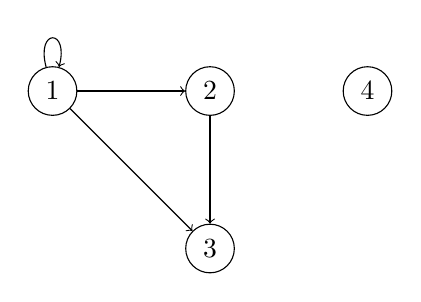
\begin{tikzpicture}[->,node distance=2cm]
  \node[draw,circle] (A) {\LR{$1$}};
  \node[draw,circle] (B) [right of=A] {\LR{$2$}};
  \node[draw,circle] (C) [below of=B] {\LR{$3$}};
  \node[draw,circle] (D) [right of=B] {\LR{$4$}};
  \draw (A) to [loop above]  (A);
  \draw (A) to  (B);
  \draw (A) to  (C);
  \draw (B) to  (C);
  \end{tikzpicture}
\intertext{\RL{دا له هغه ګراف \LR{$\tuple{V', E}$} څخه بېل دے چې
  \LR{$V' = \{1, 2, 3\}$} وي، او داسې ښکاري:}}
& 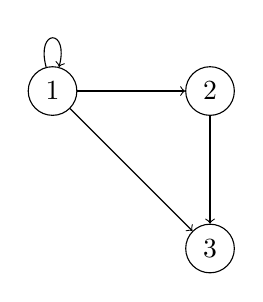
\begin{tikzpicture}[->,node distance=2cm]
  \node[draw,circle] (A) {\LR{$1$}};
  \node[draw,circle] (B) [right of=A] {\LR{$2$}};
  \node[draw,circle] (C) [below of=B] {\LR{$3$}};
  \draw (A) to [loop above]  (A);
  \draw (A) to  (B);
  \draw (A) to  (C);
  \draw (B) to  (C);
  \end{tikzpicture}
\end{align*}
\end{ex}

\begin{prob}
  په سټ \LR{$\{1, 2, 3, 4\}$} باندې د کوچني يا برابر کېدو اړيکه
  \LR{$\le$} د ګراف په توګه وګورئ او ورسره سم شکل رسم کړئ۔
\end{prob}




\olfileid{sfr}{rel}{tre}
\olsection{ونې}

د جزوي ترتيب يو خاص ډول چې د منطق په ټولو برخو کښې مهم رول لري،
\emph{ونه} ده۔ متناهي ونې د منطق په لومړنيو برخو کښې راځي:
مثلاً، فارمولونه په نحوي ونه کښې د خپلو برخو په بېلولو پوهېدلے
شو، او په ډېرو اشتقاق نظامونو کښې اشتقاقونه هم د
متناهي ونو بڼه خپلوي۔
%
نامتناهي ونې د بياني منطق او د لومړۍ درجې منطق د بشپړتيا د قضيو
په ثبوت کښې لا راڅرګندېږي، او په ټول رياضي منطق کښې کارول کېږي۔

د سټونو د نظريې د ونې مفهوم د ګرافونو په نظريه کښې د ونې له
مفهوم سره نژدې تړاو لري۔ دا د يوې (متناهي) ونې انځور دے:

\begin{center}
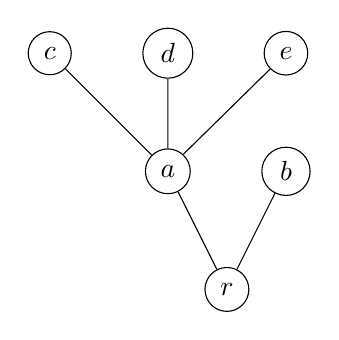
\begin{tikzpicture}[nodes={draw, circle}, -]
\node{\LR{$r$}} [grow'=up]
    child { node {\LR{$a$}}
        child { node {\LR{$c$}} }
        child { node {\LR{$d$}} }
        child { node {\LR{$e$}} }
    }
    child { node {\LR{$b$}} };
\end{tikzpicture}
\end{center}

تر ټولو لاندې غوټه \LR{$r$} ريښه ده۔ له \LR{$r$} پرته د هرې غوټې سمدستي
لاندې پوره يوه مور غوټه شته۔ که له غوټې \LR{$x$} څخه د څنډو په تعقيب
پورته تلو سره غوټې \LR{$y$} ته رسېدلے شو، نو د \LR{$x$} او \LR{$y$} ترمنځ دا
اړيکه داسې ګڼلے شو چې \LR{$x$} د \LR{$y$} يو \emph{نيکۀ} دے۔

په يوه ونه کښې د نيکۀ اړيکه سخت جزوي ترتيب دے۔ دا د سټونو د
نظريې تعريف ته لاره هواروي۔ د هغه د بيانولو دپاره دوه مفهومونو ته
اړتيا لرو۔ په سټ \LR{$A$} کښې، چې د \LR{$\le$} په ذريعه جزوي مرتب شوے وي،
\emph{تر ټولو کوچنے غړے} هغه غړے \LR{$x \in A$} دے چې د
هر \LR{$y \in A$} دپاره \LR{$x \le y$} ولرو۔ يو سټ د \LR{$\le$} په ذريعه
\emph{ښۀ مرتب} دے که هر ناتش فرعي سټ ئې تر ټولو کوچنے غړے ولري۔

\begin{defn}[ونه]
\emph{ونه} داسې جوړه \LR{$T = \tuple{A, \le}$} ده چې \LR{$A$} يو سټ وي،
او \LR{$\le$} په \LR{$A$} باندې داسې جزوي ترتيب وي چې يوازينے تر ټولو
کوچنے غړے \LR{$r \in A$} ولري (چې \emph{ريښه} بللے شي)، او د هر
\LR{$x \in A$} دپاره سټ \LR{$\Setabs{y}{y \le x}$} د \LR{$\le$} په ذريعه
ښۀ مرتب وي۔
\end{defn}

\begin{defn}[ځايناستي]
فرض کړئ \LR{$T = \tuple{A, \le}$} يوه ونه ده۔ که \LR{$x,y \in A$}،
\LR{$x < y$}، او داسې \LR{$z \in A$} نۀ وي چې \LR{$x < z < y$} وي، نو وايو
چې \LR{$y$} د \LR{$x$} \emph{ځايناستے} دے۔
\end{defn}

د \LR{$x \in A$} ځايناستي د هغې \emph{اولادونه} هم بللے شي۔ که \LR{$y$}
د \LR{$x$} ځايناستے وي، نو \LR{$x$} د \LR{$y$} \emph{مخکينے} يا \emph{مور}
بولو۔

\begin{prop}
که \LR{$\tuple{A,\le}$} يوه ونه وي، نو له ريښې پرته د هر \LR{$x \in A$}
له يوه څخه زيات مخکيني نۀ شي کېدلے۔
\end{prop}

\begin{proof}
  فرض کړئ \LR{$y_1 < x$}، \LR{$y_2 < x$} او \LR{$y_1 \neq y_2$}۔ نو
  \LR{$\{y_1, y_2\} \subseteq \Setabs{z}{z<x}$}۔ ځکه چې
  \LR{$\Setabs{z}{z<x}$} د \LR{$\le$} په ذريعه ښۀ مرتب دے، د دې فرعي سټ
  \LR{$\{y_1, y_2\}$} تر ټولو کوچنے غړے لري، چې ښکاره ده يا به \LR{$y_1$}
  وي يا \LR{$y_2$}۔ نو يا \LR{$y_1 \le y_2$} يا \LR{$y_2 \le y_1$}۔ فرض مو
  کړے و چې \LR{$y_1 \neq y_2$}، نو په حقيقت کښې يا \LR{$y_1 < y_2$} يا
  \LR{$y_2 < y_1$}۔ ځکه چې \LR{$y_1 < x$} او \LR{$y_2 < x$} مو هم فرض کړي وو،
  دا هم لرو چې يا \LR{$y_1 < y_2 < x$} يا \LR{$y_2 < y_1 < x$}۔ نو
  \LR{$y_1$} او \LR{$y_2$} دواړه د \LR{$x$} مخکيني نۀ شي کېدلے۔
\end{proof}

\begin{defn}
ونه \LR{$T = \tuple{A, \le}$} \emph{نامتناهي} بللے شي که \LR{$A$} نامتناهي
سټ وي، او که نه نو \emph{متناهي} ده۔ که په \LR{$T$} کښې هر \LR{$x \in A$}
يوازې متناهي شمېر ځايناستي ولري، نو وايو چې \LR{$T$}
\emph{متناهي څانګېدونکې} ده۔
\end{defn}

\begin{defn}[څانګې]
که ونه \LR{$T = \tuple{A, \le}$} راکړل شي، نو د \LR{$T$} يوه \emph{څانګه}
په \LR{$T$} کښې يوه اعظمي ځنځير ده؛ يعنې داسې سټ \LR{$B \subseteq A$} چې
د هر \LR{$x, y \in B$} دپاره يا \LR{$x \le y$} يا \LR{$y \le x$} وي، او د
هر \LR{$z \in X \setminus B$} دپاره داسې \LR{$u \in B$} شته چې نۀ
\LR{$z \le u$} وي او نۀ \LR{$u \le z$}۔
%
د \LR{$T$} د ټولو څانګو د سټ د ښودلو دپاره \LR{$[T]$} کاروو۔
\end{defn}

\begin{ex}
د متناهي څانګېدونکې ونې يوه مشهوره بېلګه د \LR{$0$} ګانو او \LR{$1$} ګانو
د متناهي لړيو \emph{نامتناهي دوه ګونې ونه} ده۔ کله کله په
\LR{$\{0,1\}^*$} يا \LR{$\Bin^*$} ښودل کېږي، او د غځونې د اړيکې
\LR{$\sqsubseteq$} په ذريعه مرتب شوې ده (مثلاً، \LR{$101 \sqsubseteq 101101$})۔
ځکه چې هر دوه ګونے توريز تسلسل په پاے کښې د \LR{$0$} يا \LR{$1$} په
ورزياتولو تل غځولے شو، دا ونه نامتناهي ډېر غړي لري: هر غړے \LR{$s$}
پوره دوه ځايناستي لري، \LR{$s0$} او \LR{$s1$}۔ ريښه ئې تشه لړۍ \LR{$\emptyseq$} ده۔
\end{ex}

\begin{ex}
په يو څه زياته عمومي توګه، د طبيعي عددونو د متناهي لړيو سټ
\LR{$\Nat^*$} د غځونې له اړيکې \LR{$\sqsubseteq$} سره هم يوه ونه ده۔
ښکاره ده چې دا متناهي څانګېدونکې نۀ ده: هر \LR{$s \in \Nat^*$}
نامتناهي ډېر ځايناستي \LR{$sn$} لري، د هر \LR{$n \in \Nat$} دپاره يو۔
هر \LR{$A \subseteq \Nat^*$} چې د \LR{$\sqsubseteq$} لاندې تړلے وي، د
\LR{$\Nat^*$} يوه \emph{فرعي ونه} ده۔ (يعنې \LR{$A$} داسې دے چې که
\LR{$s \in A$} او \LR{$s' \sqsubseteq s$} وي، نو \LR{$s' \in A$} هم وي۔)
ټولې متناهي ونې د \LR{$\Nat^*$} د متناهي فرعي ونو په توګه ښودل کېدلے شي۔
\end{ex}

\begin{prop}[د کونيګ مرستندويه قضيه]
که \LR{$T = \tuple{A,\le}$} متناهي څانګېدونکې نامتناهي ونه وي، نو
\LR{$T$} يوه نامتناهي څانګه لري۔
\end{prop}

د کونيګ د مرستندويې قضيې يوه خاصه بڼه چې د محاسبه کېدنې په نظريه
کښې ډېره کارېږي، \emph{د کونيګ کمزورې مرستندويه قضيه} بللے شي:
د \LR{$\{0,1\}^*$} هره نامتناهي فرعي ونه يوه نامتناهي څانګه لري۔




\olfileid{sfr}{rel}{ops}
\olsection{په اړيکو باندې عمليات}

اړيکې بدلول يا سره يوځاے کول ډېر وخت ګټور وي۔ په
\olref[sfr][rel][ord]{prop:stricttopartial} کښې مو د اړيکو
\emph{اتحاد} په پام کښې نيولے و؛ دا يوازې د دوو اړيکو اتحاد دے
چې د جوړو د سټونو په توګه ګڼل شوې وي۔ همدارنګه، په
\olref[sfr][rel][ord]{prop:partialtostrict} کښې مو د اړيکو نسبي
تفاضل په پام کښې نيولے و۔ لاندې ځينې نور عمليات دي چې په اړيکو
باندې ئې کولے شو۔

\begin{defn}\ollabel{relationoperations}
فرض کړئ \LR{$R$} او \LR{$S$} اړيکې دي، او \LR{$A$} هر يو سټ دے۔

د \LR{$R$} \emph{معکوس} دا دے:
\LR{$R^{-1} = \Setabs{\tuple{y, x}}{\tuple{x, y} \in R}$}۔

د \LR{$R$} او \LR{$S$} \emph{نسبي حاصل ضرب} دا دے:
\LR{$(R \mid S) = \{\tuple{x, z} : \exists y(Rxy \land Syz)\}$}۔

تر \LR{$A$} پورې د \LR{$R$} \emph{محدودونه} دا ده:
\LR{$\funrestrictionto{R}{A}= R \cap A^2$}۔

په \LR{$A$} باندې د \LR{$R$} \emph{تطبيق} دا دے:
\LR{$\funimage{R}{A} = \{y : (\exists x \in A)Rxy\}$}
\end{defn}

\begin{ex}
فرض کړئ \LR{$S \subseteq \Int^2$} په \LR{$\Int$} باندې د ځايناستي اړيکه
ده؛ يعنې \LR{$S = \Setabs{\tuple{x, y} \in \Int^2}{x + 1 = y}$}،
نو \LR{$Sxy$} هله او يوازې هله چې \LR{$x + 1 = y$} وي۔

\LR{$S^{-1}$} په \LR{$\Int$} باندې د مخکيني اړيکه ده، يعنې:
\LR{$\Setabs{\tuple{x,y}\in\Int^2}{x -1 =y}$}۔

\LR{$S\mid S$} دا دے:
\LR{$ \Setabs{\tuple{x,y}\in\Int^2}{x + 2 =y}$}

\LR{$\funrestrictionto{S}{\Nat}$} په \LR{$\Nat$} باندې د ځايناستي اړيکه ده۔

\LR{$\funimage{S}{\{1,2,3\}}$} دا دے: \LR{$\{2, 3, 4\}$}۔
\end{ex}

\begin{defn}[انتقالي بندښت]فرض کړئ \LR{$R \subseteq A^2$} يوه دوه ځاييزه اړيکه ده۔

د \LR{$R$} \emph{انتقالي بندښت} دا دے:
\LR{$R^+ = \bigcup_{0 < n \in \Nat} R^n$}؛ دلته په بازګشتي ډول
\LR{$R^1 = R$} او \LR{$R^{n+1} = R^n \mid R$} تعريفوو۔

د \LR{$R$} \emph{انعکاسي انتقالي بندښت} دا دے:
\LR{$R^* = R^+ \cup \Id{A}$}۔
\end{defn}

\begin{ex}
د ځايناستي اړيکه \LR{$S \subseteq \Int^2$} واخلئ۔ \LR{$S^2xy$} هله او
يوازې هله چې \LR{$x + 2 = y$} وي، \LR{$S^3xy$} هله او يوازې هله چې
\LR{$x + 3 = y$} وي، او داسې نور۔ نو \LR{$S^+xy$} هله او يوازې هله چې
د کوم \LR{$n \geq 1$} دپاره \LR{$x + n = y$} وي۔ په نورو ټکو، \LR{$S^+xy$}
هله او يوازې هله چې \LR{$x < y$} وي، او \LR{$S^*xy$} هله او يوازې هله چې
\LR{$x \le y$} وي۔
\end{ex}

\begin{prob}
وښيئ چې د \LR{$R$} انتقالي بندښت په رښتيا انتقالي دے۔
\end{prob}



\chapter*{د دې نسخې يادښتونه}
دا يادښتونه د ژباړې د نسخې له خوا زيات شوي دي؛ د اصلي متن برخه نۀ
دي۔ په اصلي متن کښې نښې پر خپل ځاے ساتل شوې دي۔

په \olref[sfr][rel][set]{sec} کښې د طبيعي عددونو د ترتيبي اړيکو په
بېلګه کښې \LR{$I$} بې له ښکاره تعريفه کارول شوے دے۔ له سياقه داسې
ښکاري چې مطلب ئې د طبيعي عددونو د عينيت اړيکه ده۔

په \olref[sfr][rel][tre]{sec} کښې د څانګې د تعريف په فورمول کښې
\LR{$X$} راغلے، خو د ونې د غړو سټ هلته \LR{$A$} نومول شوے دے۔ له سياقه
داسې ښکاري چې په دې فورمول کښې هم مطلب \LR{$A$} دے۔ دا د اصلي متن د
نښې ناڅرګندتيا ده۔

په \olref[sfr][rel][ord]{sec} او \olref[sfr][rel][ops]{sec} کښې
\LR{$R^+$} د بېلو جوړښتونو دپاره کارول کېږي: په لومړۍ برخه کښې د قطر
په ورزياتولو انعکاسي بندښت ښيي، او په دويمه کښې انتقالي بندښت۔
په هره برخه کښې بايد د هماغې برخې تعريف تعقيب شي۔

\clearpage
\begin{LTR}\latinfont
\begin{thebibliography}{1}
\bibitem[Benacerraf(1965)]{Benacerraf1965}
Benacerraf, Paul. (1965). What numbers could not be. \emph{The Philosophical Review}, 74(1), 47--73.
\end{thebibliography}
\end{LTR}
\end{document}
